% Manuscript draft -- Havana Bay: robust vs fragile conclusions about flushing
% Target: Environmental Modelling & Software (Elsevier), research article.
% Class: elsarticle (official: github.com/STM-Document-Engineering/elsarticle, 04aee43).
% EMS rules (Guide for Authors, checked 17-oct-2026): abstract <= 150 words;
% 1-7 keywords; 3-5 highlights of <= 85 characters (separate file at submission);
% graphical abstract required; data deposited in a repository and cited;
% CRediT, competing interests, funding and GenAI declaration required.
%
% RULE: every input is public and replicable. Unpublished data (CUJAE, GEOCUBA,
% tide-gauge series) may only appear as optional comparison.
% Numbers: source of truth is repos/Modelo-hidrodin-mico/docs/articulo/cifras.md
% (state of 8-nov-2026, commit 1e32fcf of the working repo).
% \prov{} = provisional value (blue); \todo{} = missing content (red).
% 14-nov: rewritten for focus (6 figures, 5 tables); removed figures stay in figuras/.
% 14-nov (review V1): headline aligned on 'one to two weeks'; tracer-protocol deviation
% declared; pilot depth and 2002 river data attributed as in the sources; DOIs completed.
% 16-nov (review V2): reframed around parametric vs structural uncertainty; heat-flux
% results moved to the centre (Fig. 7, Table 4 column); Sentinel-2 figure in main text;
% mesh, tide check and tidal prism figures added to the supplement; numerical behaviour
% moved to Text S1; Table 2 gains a 'Basis' column; unused affiliations removed.
\documentclass[a4paper,fleqn]{ems-dc}
\usepackage[authoryear]{natbib}
\usepackage{graphicx}
\usepackage{booktabs}
\usepackage{xcolor}
\usepackage{enumitem}
%\usepackage[section]{placeins}
%\usepackage{lineno}\linenumbers   % line numbers for review: uncomment
\setlength{\emergencystretch}{2em}
\setlength{\tabcolsep}{4pt}
\AtBeginEnvironment{table}{\small}
\AtBeginEnvironment{table*}{\small}
\newcommand{\todo}[1]{\textcolor{red}{[TODO: #1]}}
% Placeholder for a link Alex fills in (red, typewriter): replace the whole \ph{...}.
\newcommand{\ph}[1]{\textcolor{red}{\textsf{#1}}}
\newcommand{\prov}[1]{\textcolor{blue}{#1}}

\begin{document}
\let\WriteBookmarks\relax
\shorttitle{Flushing of Havana Bay from public data}
\shortauthors{A.M. Rivera-Rivera et al.}

\title[mode=title]{Water renewal in Havana Bay, Cuba: robust and fragile conclusions from public-data ensemble simulations}

\author[1,2,3]{Alex M. Rivera-Rivera}
\cormark[1]
\ead{alex.rivera.rivera@ulb.be}
\credit{Conceptualization, Data curation, Formal analysis, Investigation, Methodology,
Resources, Software, Validation, Visualization, Writing -- original draft, Writing --
review \& editing}
\author[3,2]{Daniela Martinez-Ortiz}
\credit{Conceptualization, Data curation, Formal analysis, Investigation, Methodology,
Resources, Software, Validation, Visualization, Writing -- original draft, Writing --
review \& editing}
\author[3]{Ernesto Altshuler}
\credit{Conceptualization, Investigation, Methodology, Project administration,
Supervision, Writing -- review \& editing}
\author[4]{Alexandre Campo}
\credit{Conceptualization, Formal analysis, Investigation, Methodology, Visualization,
Writing -- review \& editing}
\author[4]{Stamatios C. Nicolis}
\credit{Conceptualization, Formal analysis, Investigation, Methodology, Project
administration, Supervision, Visualization, Writing -- review \& editing}

\affiliation[1]{organization={Innovation Laboratory, Technological University of Havana Jos\'e Antonio Echeverr\'ia (CUJAE)},
  postcode={19390}, city={Havana}, country={Cuba}}
\affiliation[2]{organization={Facult\'e des Sciences, Universit\'e Libre de Bruxelles (ULB)},
  postcode={1050}, city={Brussels}, country={Belgium}}
\affiliation[3]{organization={Center for Complex Systems, Physics Faculty, University of Havana},
  postcode={10400}, city={Havana}, country={Cuba}}
\affiliation[4]{organization={Brussels School of Engineering, Universit\'e libre de Bruxelles},
  addressline={Avenue Franklin Roosevelt 50}, postcode={1000}, city={Brussels}, country={Belgium}}
\cortext[1]{Corresponding author}
% Authors, affiliations, CRediT roles, funding and AI statement as in the FocalReview
% manuscript (Alex, 13-nov-2026); author list as in the V2 received on 16-nov-2026.

% <= 150 words (16-nov).
\begin{abstract}
Many polluted bays lack the surveys, tide and current records to calibrate a
hydrodynamic model. We ask which conclusions about their flushing survive without them.
Havana Bay (Cuba), a 4.9~km$^2$ bay behind a 1.5~km channel, is modelled in 3D with SCHISM
from public data only; nine poorly known inputs, from nineteenth-century charts to river
discharge, are sampled in a 704-member Sobol ensemble. The tide alone renews the bay poorly;
an estuarine circulation driven by 2~m$^3$\,s$^{-1}$ of river water does. Across the
ensemble the bay-mean water age is 7.8~days (5.6--10.4, 90\% range), increases from the
channel to the inner coves in every member, and depends mostly on river discharge. One
process left out of the ensemble matters more than all nine inputs: the air--sea heat flux
roughly doubles the age, to about two weeks, and keeps it from settling. The bay is renewed
in weeks, not months.
\end{abstract}

% Highlights: 3-5 items, each <= 85 characters; also submitted as a separate file.
\begin{highlights}
\item A 3D model of Havana Bay built from public data only, run as a 704-member ensemble.
\item An estuarine circulation driven by the rivers, not the tide, renews the bay.
\item River discharge, not the old charts or the tide, controls most of the uncertainty.
\item The air--sea heat flux, left out of the ensemble, doubles the age to two weeks.
\item The ensemble spread understates the uncertainty when one process is missing.
\end{highlights}

\begin{keywords}
water age \sep residence time \sep ensemble modelling \sep global sensitivity analysis \sep
structural uncertainty \sep historical nautical charts \sep Havana Bay
\end{keywords}

\maketitle

%======================================================================
\section{Introduction}\label{sec:intro}
%======================================================================
Semi-enclosed bays collect the waste of the cities around them, and how long their water
stays inside largely decides how much of that load becomes a water-quality problem.
Flushing time, residence time and water age are the usual ways to express this
\citep{Monsen2002,Deleersnijder2001,Lucas2020}. Computing them well normally needs a
calibrated hydrodynamic model, and calibration needs bathymetry, water levels and currents
that many bays in the Global South do not have. Recent studies therefore build such models
from satellite and reanalysis data alone \citep{Payandeh2026} or calibrate them on very few
measurements \citep{RodriguesDoAmaral2025}.

The usual response to missing data is to build one model from whatever can be found and to
report one residence time. That number is hard to defend: it carries every guess made along
the way, and the reader cannot tell which conclusions rest on which guess
\citep{Uusitalo2015}. A variance-based sensitivity analysis over a large ensemble
\citep{Sobol2001,Saltelli2008,Saltelli2010} solves part of the problem, because it explores
all uncertain inputs together rather than one at a time
\citep{Saltelli2019,Pianosi2016,Razavi2021}. It cannot solve the rest. An ensemble varies the
inputs of one model structure, and the processes that the structure leaves out, or
represents too simply, are a separate source of uncertainty that no amount of input
sampling reveals \citep{Walker2003,Refsgaard2006,Gupta2012}.

We therefore treat the two kinds of uncertainty separately. Every poorly known input is
sampled in a large Sobol ensemble, which shows which conclusions hold whatever the unknown
inputs are. The main simplifications of the model are then tested one at a time, outside the
ensemble, to see whether those conclusions also survive a different model structure. To keep
the study reproducible, every input is public and free.

Havana Bay is a demanding test case. Its sediments record metal pollution
\citep{DiazAsencio2011}, and its benthic fauna lives under chronic, heavy pollution
\citep{Armenteros2009}. To our knowledge, it has been modelled only for coastal flooding
and wave overtopping along the Malec\'on \citep{PoncePortela2016,CordovaDeHorta2025}, and
no peer-reviewed study has quantified how its water is renewed. The executive summary of a
sewerage master plan gives a freshwater retention time of about four months, with little
exchange with the sea, but does not say how this was obtained \citep{JICA2004}. The only
open bathymetry inside the bay comes from two nineteenth-century editions of one nautical
chart.

We ask four questions:

\begin{enumerate}[label=(\arabic*),leftmargin=2.2em,itemsep=0pt]
\item what drives the exchange with the sea: the tide, the wind or density differences;
\item how long water stays in each part of the bay, and which of these answers survive the
missing data;
\item which unknown input controls most of the remaining uncertainty, and therefore what
should be measured first; and
\item whether the answers change when a process left out of the ensemble is added.
\end{enumerate}

\noindent The procedure is as much the contribution as its answers for Havana Bay. It uses
only public data and open-source code, fixes the conclusions to be tested before computing
them, and can be repeated in other bays that have no surveys or gauges. The answer to the
fourth question also shows, in numbers, how far the spread of a parametric ensemble can
understate the uncertainty when one structural choice dominates.

%======================================================================
\section{Study area and data}\label{sec:area}
%======================================================================
Havana Bay (Fig.~\ref{fig:map}) is a pocket bay of 4.91~km$^2$. Its entrance channel,
1530~m long and 220--330~m wide, opens to the north-west and is 12.8~m deep according to
the harbour pilots \citep{Practicos2018}. Three coves branch off a main basin 9--13~m deep:
Marimelena to the east, Guasabacoa to the south and Atar\'es to the south-west, all mostly
shallower than 4~m on the historical charts. The bay holds 26--36~hm$^3$ of water, depending
on how much of the dredging reported by the harbour pilots is applied
(Section~\ref{sec:bathy}). The often quoted mean depth of 9~m and volume of 47~hm$^3$
\citep{JICA2004} agree with neither the charts nor the pilots' depths.

The tide is small and mixed, as in much of the Caribbean region \citep{Kjerfve1981}. Off
the mouth, two independent global models give M2 amplitudes of 12.2 and 12.6~cm, K1 of 8.3
and 8.0~cm and O1 of 8.8 and 8.4~cm \citep{FES2022,HartDavis2021}, so diurnal and
semidiurnal constituents are of similar size (form factor $(K_1+O_1)/(M_2+S_2)$ of
1.0--1.05; \citealt{Pugh2014}). The mean range is about 0.29~m \citep{JICA2004}.

Three rivers enter the bay: the Luyan\'o (1.33~m$^3$\,s$^{-1}$) and the Mart\'in P\'erez
(0.72~m$^3$\,s$^{-1}$) into Guasabacoa, and the Arroyo Tadeo (0.09~m$^3$\,s$^{-1}$) into
the southern shore of Marimelena. These 2.14~m$^3$\,s$^{-1}$ are a single set of values
dated August 2002 (CIMAB) and reported by \citet{JICA2004}; the rivers have no permanent
gauging. No river reaches Atar\'es in OpenStreetMap, although drains discharge there, and
urban and industrial sewage adds a load that nobody has quantified \citep{JICA2004}.

\begin{figure*}[!t]
\centering
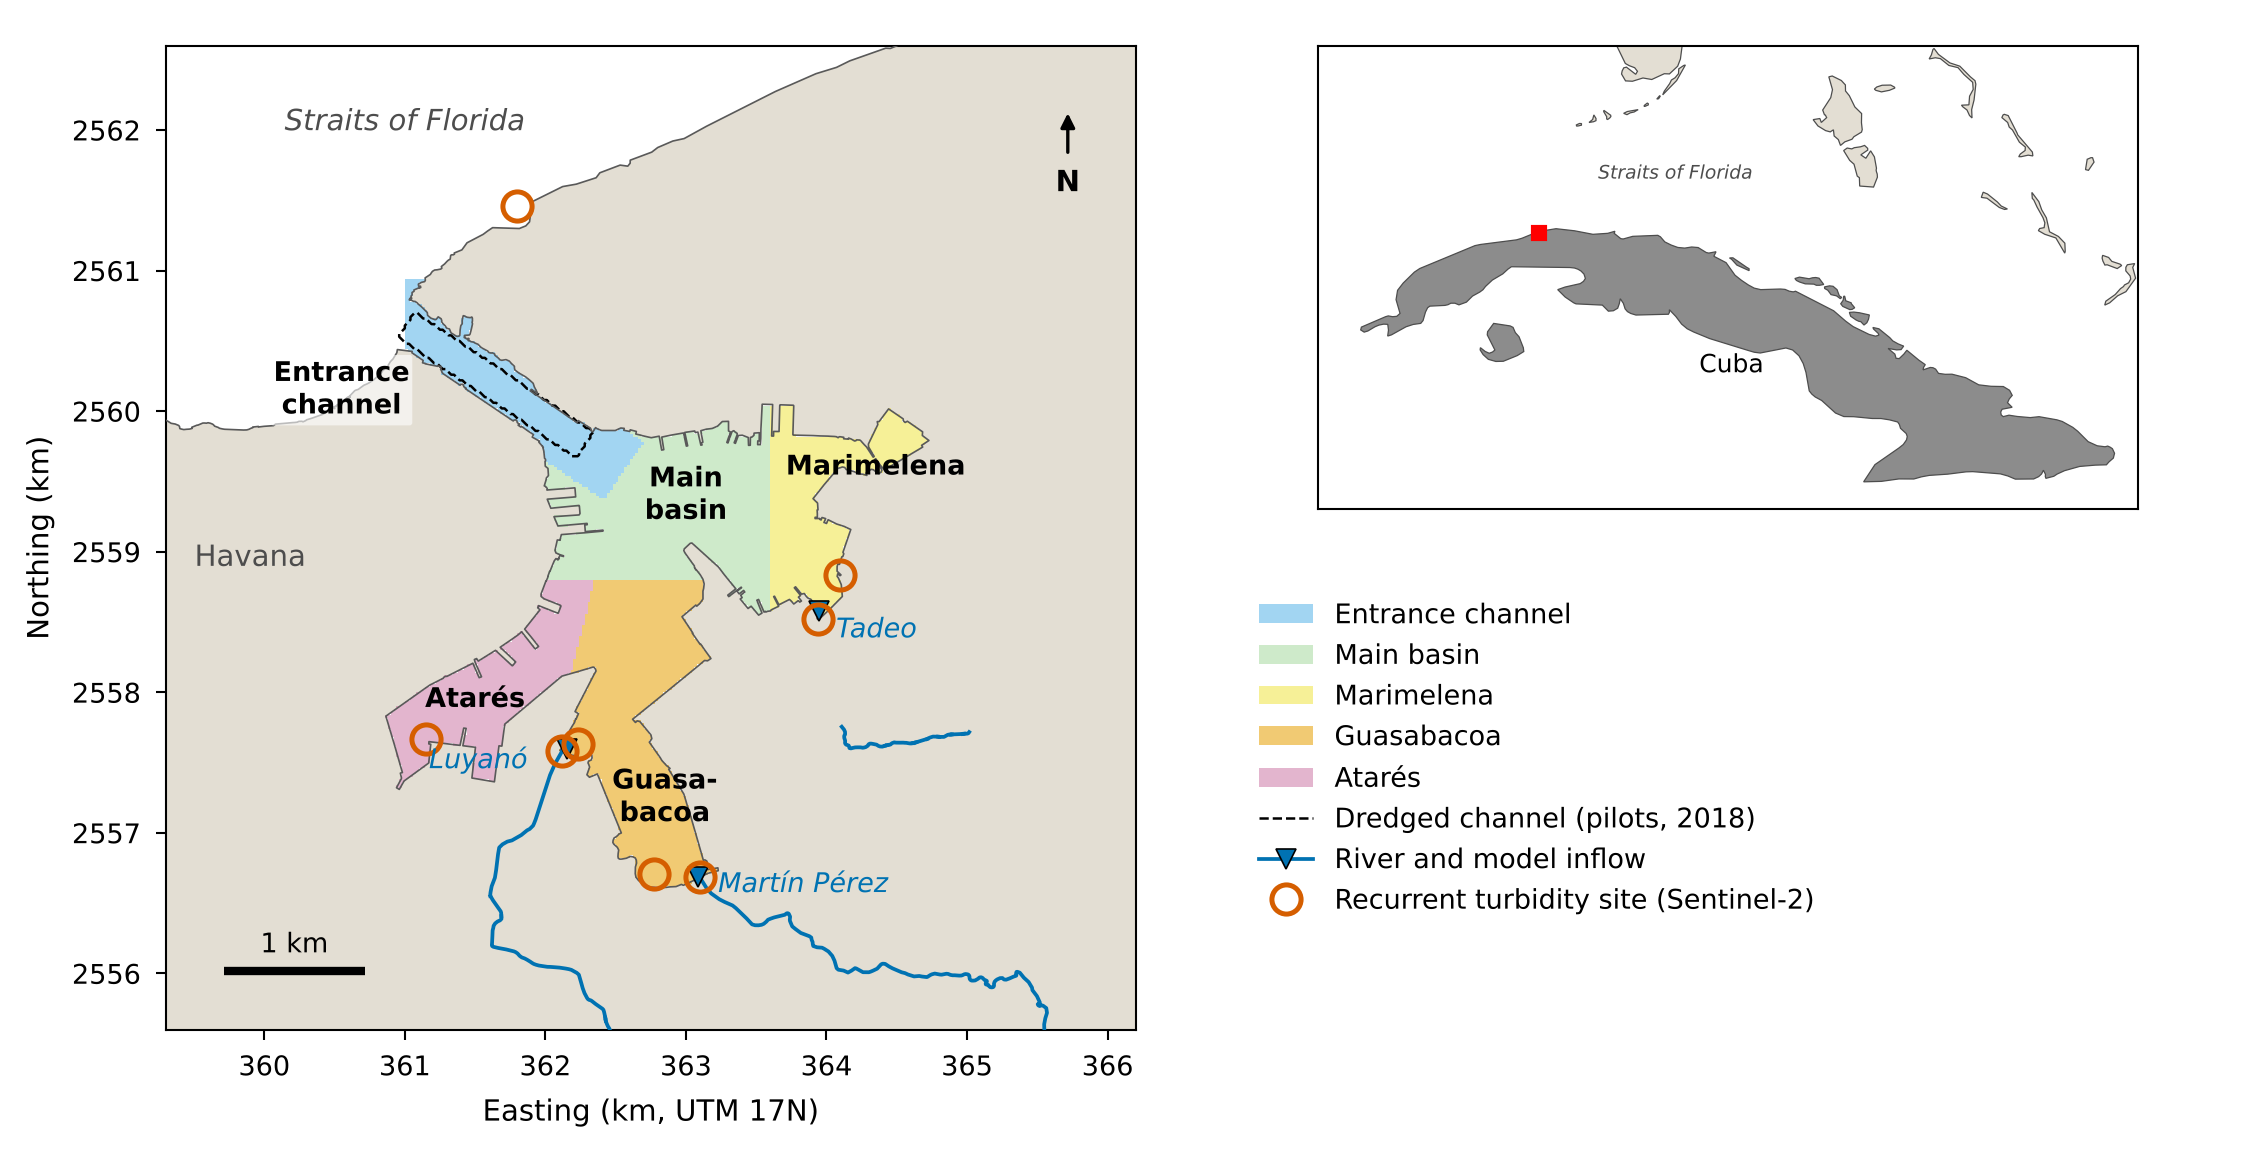
\includegraphics[width=\textwidth]{figuras/fig01_map.png}
\caption{Havana Bay: entrance channel, main basin, coves, river mouths and the five
analysis zones. Orange circles mark the foci listed by the Sentinel-2 study
(\ph{link\_sentinel2}): one preregistered candidate site (entrance channel), three
exploratory foci chosen after seeing the data, and four river or drain mouths from
OpenStreetMap; none is a validated discharge site. Blue triangles are the model river
inflows. The dashed outline is the channel dredged to the depth reported by the harbour
pilots \citep{Practicos2018}. Inset: location in Cuba (Natural Earth, public domain). Map
lines delineate study areas and do not necessarily depict accepted national
boundaries.}\label{fig:map}
\end{figure*}

Every input is public (Table~\ref{tab:data}); none requires an agreement, a purchase or a
personal contact. FES2022 needs a free account and is used only as a check; all simulations
are forced with EOT20, which needs no registration. Each download is logged with its date
and checksum in the code repository.

\begin{table*}[!t]
\centering\small
\caption{Inputs of the model and of its evaluation. All are public.}\label{tab:data}
\begin{tabular}{p{3.0cm}p{9.8cm}p{4.0cm}}
\toprule
Input & Source & Role\\
\midrule
Bathymetry inside the bay & U.S. Hydrographic Office chart No.~307, \emph{Harbor of
Havana}, from Spanish surveys to 1879 (ed.~1889) and to 1887 (ed.~1898)
\citep{USHO1889,USHO1898}; 1126 and 1514 digitised soundings & Ensemble input\\
Entrance channel and quays & Harbour-pilot depths \citep{Practicos2018} & Dredging state\\
Offshore bathymetry & GEBCO 2026 grid \citep{GEBCO2026} & Outer domain\\
Coastline, river mouths & OpenStreetMap \citep{OSM} & Fixed\\
Atmosphere & ERA5 hourly, 2016--2025 \citep{Hersbach2020} & Forcing; wind perturbed\\
Tide & EOT20, 9 constituents \citep{HartDavis2021} & Boundary; amplitude perturbed\\
Tide (comparison) & FES2022, 11 constituents \citep{FES2022,Lyard2026} & Check of EOT20\\
River flows & Values of August 2002 (CIMAB), in \citet{JICA2004} & Ensemble input\\
Sea-surface temperature & NOAA OISST v2.1, daily \citep{Huang2021} & Structural tests\\
Turbidity persistence & Sentinel-2, 2017--2025 (\ph{link\_sentinel2}) & Evaluation only\\
Model & SCHISM \citep{Zhang2016} & Open source\\
\bottomrule
\end{tabular}
\end{table*}

%======================================================================
\section{Methods}\label{sec:methods}
%======================================================================
\subsection{Bathymetry from a nineteenth-century chart}\label{sec:bathy}
The two editions of chart No.~307 record independent Spanish surveys inside the bay, one to
1879 and one to 1887. Lead-line soundings of this kind have been used to reconstruct past
bathymetry and to model how estuaries have changed \citep{Jaffe2007,Ralston2019,Poirier2020}.
We digitised their soundings by hand (Fig.~\ref{fig:soundings}), converting fathoms to
metres, from a georeferenced scan of the 1889 edition (RMS error 18~m) and from the 1898
edition registered onto it (median residual 1.2~m). The charts do not give their vertical
datum, so we treat it as an uncertain offset of 0 to +0.5~m.

The soundings were interpolated onto a 20~m UTM grid, with the OpenStreetMap coastline at
zero depth and GEBCO blended in 150--600~m away from the nearest sounding. Where both
surveys have soundings, their differences show no bias and a mean absolute value of
0.76~m. Treating the chart error as a spatially correlated field \citep{Plant2002,Cea2012},
a variogram fitted to 12\,134 of these differences gives $\sigma = 0.9$~m with a correlation
length $L = 150$~m. We use these values, taken from the data rather than assumed, to add a
Gaussian random field to each ensemble member; the field fades towards the shore and leaves
the maintained channel untouched.

The bay has been dredged since the surveys, and dredging can change the dynamics of an
estuary substantially \citep{Ralston2019}. A dredging state $\alpha$ between 0 and 1 moves
each member from the chart as surveyed ($\alpha = 0$) to a present-day estimate
($\alpha = 1$): the entrance channel at least 12.8~m deep along its 220~m~$\times$~1530~m
alignment, and the historically navigable water (at least 5~m deep and connected to the
channel) at 11~m, within the 9.75--11.58~m given by the harbour pilots
\citep{Practicos2018}. The bay volume then spans 26--36~hm$^3$, while the random field adds
only $\pm 1$~hm$^3$ (Fig.~\ref{fig:bathy}).

\begin{figure*}[!t]
\centering
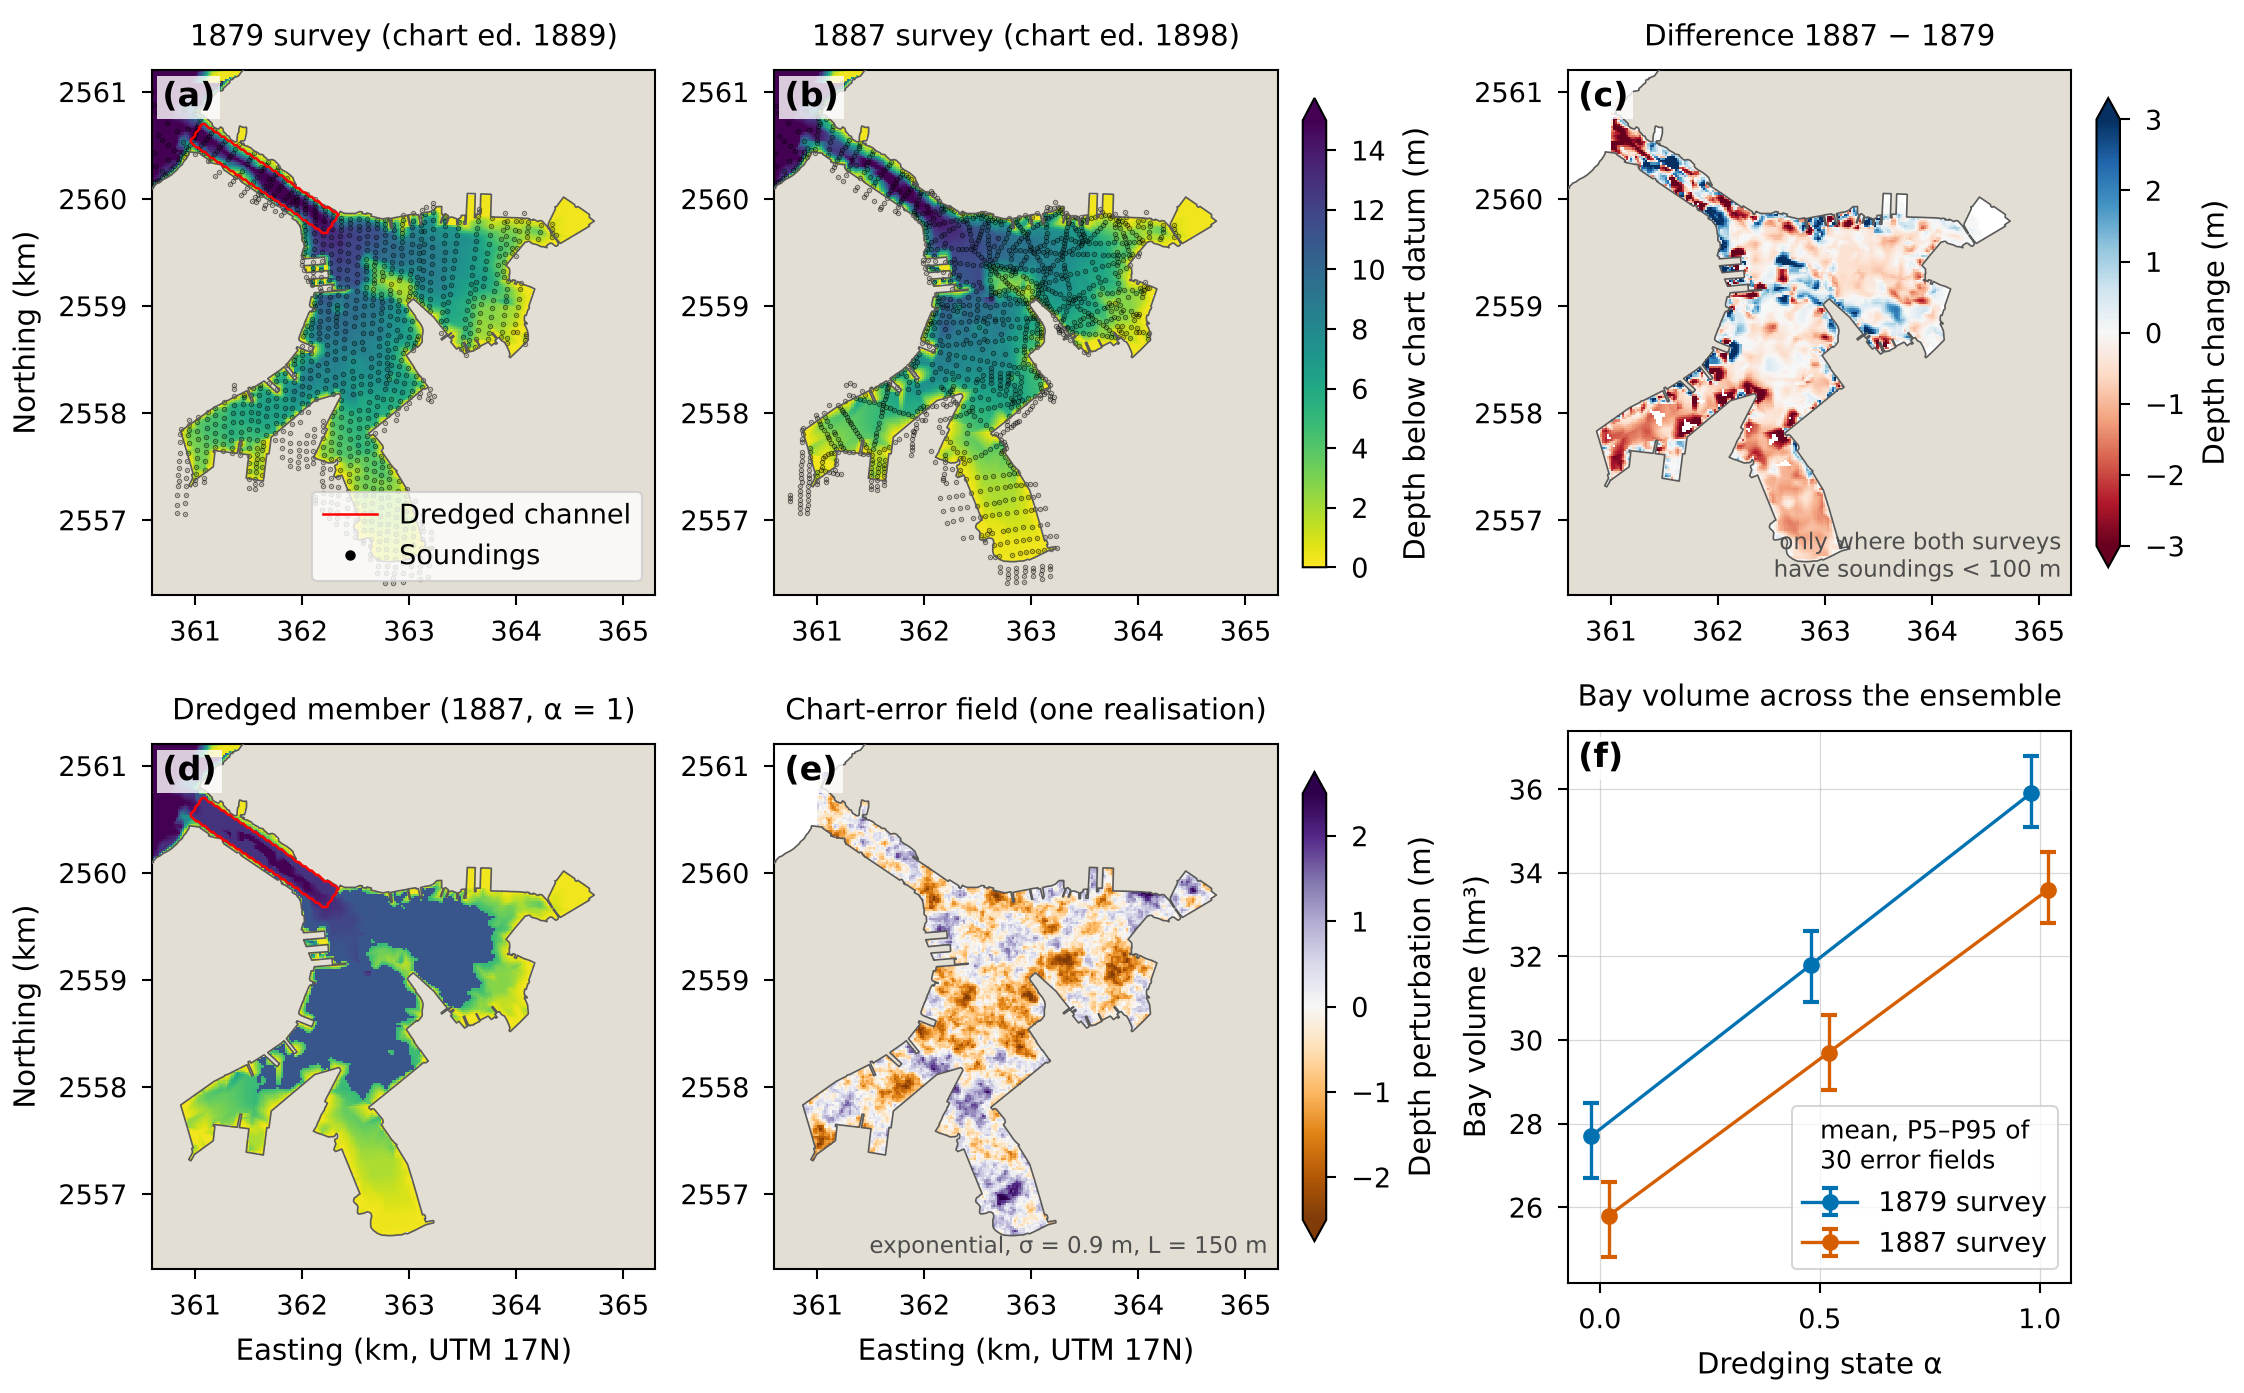
\includegraphics[width=\textwidth]{figuras/fig02_bathymetry.png}
\caption{Bathymetry from chart No.~307 and its uncertainty. (a, b) Interpolated surfaces
and soundings of the 1879 survey (chart edition of 1889) and of the 1887 survey (edition of
1898); the red rectangle is the dredged channel. (c) Difference between the surveys, shown
only where both have soundings within 100~m. (d) Ensemble member with the 1887 survey and
the dredged state ($\alpha=1$). (e) One realisation of the chart-error field. (f) Bay volume
against dredging state for both surveys (mean and P5--P95 of 30 error
fields).}\label{fig:bathy}
\end{figure*}

\subsection{Model and forcing}\label{sec:model}
We use SCHISM \citep{Zhang2008,Zhang2016} (commit 09f407e8) in three dimensions, with 16
terrain-following levels, a 100~s time step, the $k$--$kl$ form of the generic length-scale
turbulence closure \citep{Umlauf2003,Warner2005} and Coriolis forcing. The unstructured
mesh, built with DistMesh \citep{Persson2004} on a 5~km circle centred on the bay mouth, has
4832 nodes and 8941 triangles: 25~m elements in the entrance channel (about 11 across it),
40~m in the bay and up to 400~m offshore (Fig.~\ref{fig:mesh}). The open boundary is a
33-node arc in 46--1220~m of water. Momentum advection is switched off within 800~m of it, a
friction sponge ($C_d \to 0.05$) is applied within 1~km, and the wind stress is ramped up
from zero at the boundary to its full value at 2~km; removing the sponge changed velocities
at the boundary by a factor of two but left levels and currents inside the bay unchanged to
the first decimal.

In the ensemble, density depends on salinity only. River water enters with zero salinity,
the open boundary is held at a salinity of 36 and a temperature of 28~$^\circ$C, and there
is no air--sea heat flux, evaporation or precipitation; the heat flux is tested separately
(Section~\ref{sec:extra}). Hourly ERA5 wind, pressure, air temperature, humidity, radiation
and precipitation drive the surface \citep{Hersbach2020}. ERA5 surface winds have known
biases \citep{BelmonteRivas2019}, and ERA5 has only $3 \times 4$ grid points over the area,
which is why the wind enters the ensemble with a speed factor and a direction rotation. The
open-boundary tide is built from the nine EOT20 constituents with nodal corrections
\citep{Pugh2014}. FES2022 differs from it by at most 0.4~cm in every constituent amplitude
off the mouth and by 1.15~cm RMS in predicted water level (Fig.~\ref{fig:tide}), well
inside the $\pm10\%$ amplitude range of the ensemble. The rivers enter at the mesh elements
nearest their OpenStreetMap mouths, with the 2002 flows multiplied by the ensemble discharge
factor. All simulations start on 1 January 2016 and cover the dry season. The year was
chosen without a particular criterion, after a first look at the 2016--2025 period of the
ERA5 download and before any ensemble member was run.

\subsection{Water age and the other metrics}\label{sec:metrics}
Water age is computed with the age tracer of \citet{Deleersnijder2001} \citep[see
also][]{Delhez1999} as implemented in SCHISM, an approach widely used in estuaries
\citep{Shen2004}, following the definitions of \citet{Monsen2002}. Sea water and river
water both enter with age zero, so age is the time since the water entered the bay by
either route; it is not a freshwater retention time. To compare with the only earlier
estimate we also compute the freshwater flushing time $T_f = V_f/Q$
\citep{Alber1999,Sheldon2002}, where $V_f$ is the fresh water in the bay, from $1 - S/36$,
and $Q$ the river discharge. This needs full output fields, which are kept for a few runs
only.

Fields are written every 4~h. Each 120-day member is summarised over its last 30 days in
five zones (Fig.~\ref{fig:map}: channel, main basin, Marimelena, Guasabacoa, Atar\'es) and
in the whole bay. The main metric is the mean age of a zone, a volume-weighted mean over all
its nodes and levels and over the 30 days. We also store percentiles, the volume fraction
older than 30 days, surface and bottom age maps, the surface freshwater fraction, and
surface fields at 16:00~UTC, the output nearest to the Sentinel-2 overpass
(16:16--16:17~UTC), interpolated to the 20~m grid of the satellite study. A member is in
equilibrium if its bay-mean age changes by at most 0.05~d per day over its last 10 days.
This criterion presumes forcing that changes little over the window; with the air--sea heat
flux it does not, and for those runs we report 30-day means and their range. The discharge
through the channel is computed but not used: from 4-hourly velocities its net value has an
error of about $\pm 6$~m$^3$\,s$^{-1}$, more than the river inflow.

In the spirit of preregistration \citep{Nosek2018}, the metrics, thresholds and conclusions
to be tested were written down, dated and kept under version control before the results
they govern existed: the Sentinel-2 comparison on 21 October 2026 and the ensemble metrics
on 27 October 2026, before any member had started. Later changes are logged in them with
their dates. We depart from the metrics protocol in two places. It asked for the volume
fractions older than 7 and 14 days, which were not stored, so for those thresholds we report
the probability across members instead. And the freshwater flushing time was added
afterwards, only to compare with the earlier estimate (Section~\ref{sec:jica}).

\subsection{The ensemble and the conclusions fixed in advance}\label{sec:ensemble}
Nine uncertain inputs (Table~\ref{tab:params}) are sampled with a Saltelli design
\citep{Saltelli2002} on a randomised Sobol sequence. With a base sample of $N = 64$ and
$d = 9$ inputs this gives $N(d+2) = 704$ members of 120 days each. First-order ($S_1$) and
total ($S_T$) Sobol indices are estimated with the Jansen estimators
\citep{Jansen1999,Saltelli2010}, with 95\% intervals from 1000 bootstrap resamples
\citep{Archer1997}; the code recovers the analytical indices of the Ishigami function
\citep{Ishigami1990} within $\pm 0.02$. With $N = 64$ the sampling error is about 0.1 for
total and 0.2 for first-order indices, so we read mainly the total ones. The 120-day length
comes from the mechanism runs: with rivers, the bay-mean age settles after about 30 days,
which leaves room for members with little river water.

\begin{table*}[!t]
\centering
\caption{Uncertain inputs of the ensemble and the basis of each range. The river discharge
factor multiplies the 2.14~m$^3$\,s$^{-1}$ of the 2002 values.}\label{tab:params}
\begin{tabular}{llll}
\toprule
Input & Range & Distribution & Basis\\
\midrule
Chart survey & 1879 or 1887 & Discrete & Two editions of chart No.~307\\
Dredging state $\alpha$ & 0--1 & Uniform & Chart as surveyed to pilots' depths\\
Chart error ($\sigma = 0.9$~m, $L = 150$~m) & Realisation & Random seed & Variogram of
survey differences\\
Vertical datum offset & 0 to +0.5~m & Uniform & Datum not stated; likely low water\\
Bottom drag coefficient $C_d$ & 0.001--0.005 & Log-uniform & No current data to calibrate\\
Wind speed factor & 0.8--1.2 & Uniform & Near-surface biases of ERA5\\
Wind direction rotation & $\pm 15^\circ$ & Uniform & Coarse ERA5 grid, no local record\\
Tidal amplitude factor & 0.9--1.1 & Uniform & Much wider than EOT20--FES2022 difference\\
River discharge factor & 0.25--2 & Log-uniform & One wet-season set of values, no gauges\\
\bottomrule
\end{tabular}
\end{table*}

The ranges of Table~\ref{tab:params} reflect what is and is not known. The survey, the
chart error and the dredging state come from the data (Section~\ref{sec:bathy}). The
vertical datum is not stated on the charts and is most likely a low-water datum, so the
offset spans 0 (soundings referred to mean sea level) to +0.5~m, more than the mean tidal
range of 0.29~m \citep{JICA2004} and than the mean lower low and lower high waters of 0.1
and 0.4~m given by the harbour pilots \citep{Practicos2018}. The bottom-drag coefficient
spans a factor of five because no current measurements exist in the bay. The wind factors
are our choice for a reanalysis with known near-surface wind biases
\citep{BelmonteRivas2019}, at a coastal site with no local wind record. The river discharges
are a single set of values dated August 2002, in the rainy season; since the simulated
window is in the dry season, we treat them as an order of magnitude and sample a factor of
0.25--2 around them (0.54--4.3~m$^3$\,s$^{-1}$ in total).

The qualitative conclusions to test were fixed in the metrics protocol and are listed, with
their outcome, in Table~\ref{tab:concl}. Each is checked on the $2N = 128$ independent
members of blocks A and B of the design. A conclusion is \emph{robust} if it holds in at
least 90\% of them, \emph{fragile} if it holds in 10--90\% and \emph{rejected} if it holds
in at most 10\%.

\subsection{Runs outside the ensemble}\label{sec:extra}
Three sets of runs use a central member: the 1887 survey, $\alpha = 0.5$, no random field,
datum offset +0.25~m, $C_d = 0.0025$, no wind or tide perturbation and the 2002 river flows.

\emph{Mechanism.} The central member is run for the whole of 2016 three times: with the tide
only; with tide and wind; and with tide, wind, rivers and density.

\emph{Model structure.} Because density turned out to drive the exchange, five 120-day runs
with rivers change one structural choice at a time: (1) the $k$--$\varepsilon$ closure;
(2) 32 instead of 16 levels; (3) a ten times larger minimum vertical diffusivity
($10^{-5}$~m$^2$\,s$^{-1}$); (4) the ERA5 air--sea heat flux with the open boundary at
28~$^\circ$C; and (5) the same heat flux with the daily NOAA OISST temperature
\citep{Huang2021} at the boundary and as initial condition. In January--April 2016 OISST off
the bay ranged from 24.5 to 27.9~$^\circ$C, so the fixed boundary of run (4) was up to
3.5~$^\circ$C too warm. Because the heat flux turned out to matter, two later tests, each
with its reading fixed before the runs, followed: the base run and runs (4) and (5) were
extended to the whole of 2016, and 16 members of block A were rerun for January--April with
the heat flux and the OISST temperature.

\emph{River tracers.} To follow each river, we add three passive tracers, one per river,
that enter with concentration 1 with their own river and 0 everywhere else. The
concentration $C_i$ at a point is then the fraction of the water that comes from river $i$.
Over the last 30 of 120 days we compute the renewal time of each river's water,
$T_i = M_i/Q_i$, where $M_i$ is the volume of that river's water in the bay and $Q_i$ its
discharge, and the share of $M_i$ found in each zone. Four cases change one thing with
respect to the central member: T0, nothing; T1, river discharge $\times0.25$; T2, discharge
$\times2$; and T3, the heat flux with OISST temperature, the largest threat found to a
density-driven circulation. The protocol, with four conclusions (R1--R4 in
Table~\ref{tab:concl}), was fixed on 8 November 2026, before any case was run. We had seen
one preview beforehand, of the surface water of the three rivers together in the central
member, in which Atar\'es gets little river water; R2 was written knowing this. A conclusion
is robust if it holds in all four cases.

Two checks were set in advance. The tracer module must reproduce the reference run, and it
does: mean age and fresh water in case T0 differ by 0.08--0.18\%. And the sum of the three
tracers must match the fresh water derived from salinity within 5\% of the bay inventory.
This second check failed in one case (T1, 5.4\%; T0, 2.2\%; T2, 0.5\%; T3, 0.6\%), which
under the protocol would void all tracer results. We could not trace the mismatch to the
flux limiter, the source injection or the restarts. Tightening the transport-solver
tolerance by five orders of magnitude moved it in either direction (T0, 4.4\%; T1, 1.7\%;
T2, 8.5\%; T3, 5.8\%), changed $T_i$ by $-21$ to $+24$\%, which stays below 7~days, and did
not change whether R1--R4 hold in any case. The cause remains unidentified, and neither
tolerance is the correct one. Keeping the tracer results is therefore a deviation from the
protocol, which we declare here: having seen these results, the first author decided to
keep T1 with its original values, without changing the threshold or the rule. We treat the
mismatch as numerical uncertainty, up to about $\pm20$\% in $T_i$ and about 5\% in water
age, and report only conclusions that hold with both tolerances.

\subsection{Checks without local observations}\label{sec:eval}
No local measurement is used to calibrate the model, so we rely on independent checks: an
analytical tidal-prism estimate; the agreement of two tide models; the insensitivity of the
results to restarts and to the open boundary; the earlier four-month estimate
\citep{JICA2004}, keeping in mind that it is not the same quantity as water age; and the
persistence of turbidity in Sentinel-2 images.

\emph{Tidal prism.} Before any model run, a Monte Carlo version ($2\times10^5$ samples) of
the classical tidal-prism estimate \citep{Fischer1979,Sanford1992} gives the renewal that
the tide alone could deliver. Bay area, depth, channel cross-section, return-flow factor and
river inflow are drawn from triangular distributions (Table~\ref{tab:prismS}), and the tide
from real days of a year synthesised from the nine EOT20 constituents. Since the tide is
mixed, most days have two floods of different size (1.93 per day on average), so the prism
is counted per day, from the larger flood, whose range has a median of 0.33~m
(0.18--0.50~m).

\emph{Sentinel-2.} Turbidity in coastal waters can be retrieved from optical satellite data
\citep{Dogliotti2015}, and Sentinel-2 provides it at 10--60~m resolution \citep{Drusch2012}.
The satellite field is the frequency with which each 20~m pixel shows a positive turbidity
anomaly in the 2017--2025 archive of a companion study (\ph{link\_sentinel2}), which defines
the anomaly and the scene selection and is published separately. We keep pixels that are
water in both masks, lie at least two pixels from the coast (a two-step erosion of the
water mask, which keeps pixels whose centre is at least 44.7~m from the nearest land pixel)
and have at least 50 valid scenes (of the 113 scenes accepted out of 637 acquisitions). The
model field is the surface freshwater fraction at 16:00~UTC, averaged over the last 30 days,
in the mechanism run with rivers; a secondary test uses surface age in the runs without
rivers. The statistic is Spearman's $\rho$ \citep{Spearman1904}, with a 95\% interval from a
block bootstrap \citep{Kunsch1989} (200~m~$\times$~200~m blocks, 1000 resamples), and the
prediction is $\rho > 0$. Smooth fields can correlate by chance
\citep{Clifford1989,Lennon2000}, so we registered a control before running the comparison:
999 cyclic shifts of the satellite map by at least 500~m, which keep the spatial structure
of both maps but break their alignment. Model and satellite cover different years, and the
satellite field pools dry-season and wet-season scenes (71 and 42), so only climatological
patterns are compared.

\subsection{Computation}\label{sec:res-model}
All runs used the Lemaitre4 cluster of the C\'ECI consortium (Belgium), with seven cores per
member, four for computation and three for output. Members advance in 20-day segments
chained by hot-starts, which change the summary metrics by at most 0.01\%; the 704 members
took about $5.4\times10^4$ core-hours (76 per member). All of them completed 120 days. Of
the 128 members of blocks A and B, 117 meet the equilibrium criterion, and every class
reported below is the same with or without the other 11. Spurious speeds appear at the
open boundary and at a few very shallow nodes inside the bay; they are unrelated to the
bay-mean age, and removing the affected members changes no class (Text~S1,
Fig.~\ref{fig:boundary}).

%======================================================================
\section{Results}\label{sec:results}
%======================================================================
\subsection{The tide alone barely renews the bay}\label{sec:res-mech}
The tidal-prism estimate looks reassuring at first: if the tide did all the work, the bay
would be renewed in about three weeks (24~days, 14--47~days between the 5th and 95th
percentiles; 11.6~days if no water came back; Fig.~\ref{fig:prisma}). The catch is in the
channel. The tidal excursion there is 630~m (340--960~m), shorter than the 1530~m channel in
every sample and at most 0.63 of its length in 95\% of them. Water that leaves the bay on
the ebb does not clear the channel before the flood brings it back, so the estimate rests on
a return-flow factor that is large and unknown \citep{Sanford1992}.

The model confirms this and shows what does the work instead (Fig.~\ref{fig:mech}). With
the tide alone, the bay-mean age after one year is 166~days and still rising by 0.36~d per
day, with water older than 200~days in the coves: the same water moves back and forth. Wind
helps, bringing the bay-mean age down to 97~days, close to equilibrium. The rivers change
the picture. With their 2.14~m$^3$\,s$^{-1}$ of fresh water, the bay-mean age drops to
6.6~days and settles after about a month. The fresh water drives a gravitational circulation
\citep{Hansen1965,MacCready2010,Geyer2014}: fresh water leaves at the surface while sea
water enters near the bottom, and over the last 30 days of the year the surface water in the
channel is 6.5~days old and the bottom water 1.9~days. Dividing the bay volume of the
central member by its mean age gives an exchange of about 50~m$^3$\,s$^{-1}$, some 25 times
the river inflow itself. The order of the zones, channel $<$ basin $<$ Guasabacoa $<$
Atar\'es, is the same in the three runs; only Marimelena moves, from oldest with the tide
alone to the middle of the pack once wind or density are included.

\begin{figure*}[!t]
\centering
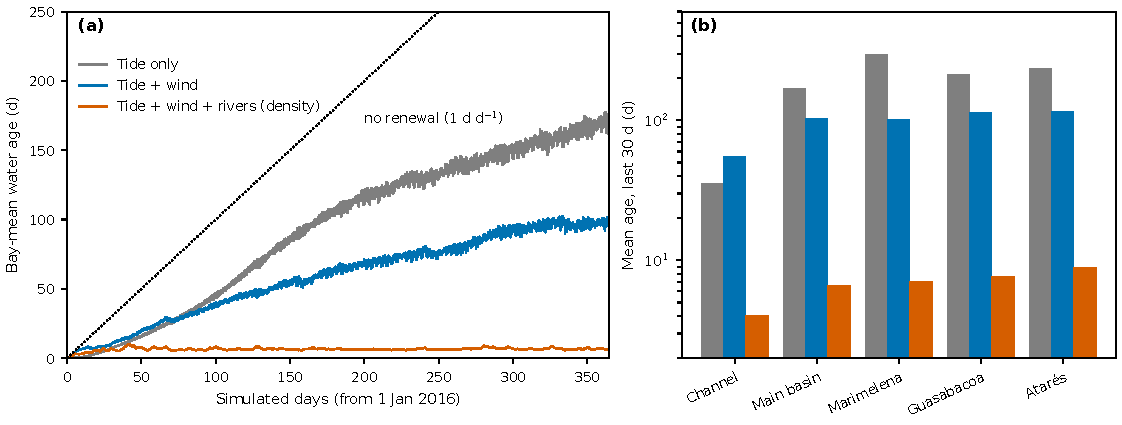
\includegraphics[width=\textwidth]{figuras/fig_mechanism.pdf}
\caption{Bay-mean water age in the three mechanism runs, 2016. (a) Daily series over one
year; the dotted line is the age of water that is never renewed. (b) Volume-weighted mean
age of each zone over the last 30 days (logarithmic axis); grey, tide only; blue, tide and
wind; orange, tide, wind and rivers.}\label{fig:mech}
\end{figure*}

\subsection{About a week within the ensemble, older towards Atar\'es}\label{sec:res-map}
Across the ensemble the bay is renewed in about a week, but not reliably faster
(Table~\ref{tab:ens}, Fig.~\ref{fig:ens}). The median bay-mean age is 7.8~days (5.6--10.4
between the 5th and 95th percentiles). It exceeds 7~days in 68\% of the members and 14 or
30~days in none. The channel, the main basin, Guasabacoa and Atar\'es age in that order in
every member, with medians from 4.6~days in the channel to 10.5~days in Atar\'es, and
Atar\'es is the only zone where some members pass two weeks (11\%). At the surface, water
older than a week is likely almost everywhere except in the outer channel, while water older
than two weeks shows up only towards the head of Atar\'es (Fig.~\ref{fig:ens}b,c).

\begin{table}[!t]
\centering\small
\caption{Mean water age (days) over the last 30 of 120 days in the ensemble: median and
P5--P95 over the 128 members of blocks A and B, and probability that the zone mean age
exceeds 7, 14 and 30 days.}\label{tab:ens}
\footnotesize\setlength{\tabcolsep}{4pt}
\begin{tabular}{@{}lrrrr@{}}
\toprule
Zone & Age (P5--P95) & $>7$~d & $>14$~d & $>30$~d\\
\midrule
Channel & 4.6 (3.2--6.4) & 0.02 & 0 & 0\\
Main basin & 7.7 (5.6--10.2) & 0.69 & 0 & 0\\
Marimelena & 8.1 (6.3--10.4) & 0.82 & 0 & 0\\
Guasabacoa & 9.1 (6.4--12.5) & 0.85 & 0 & 0\\
Atar\'es & 10.5 (7.3--14.6) & 0.96 & 0.11 & 0\\
Whole bay & 7.8 (5.6--10.4) & 0.68 & 0 & 0\\
\bottomrule
\end{tabular}
\end{table}

\begin{figure*}[!t]
\centering
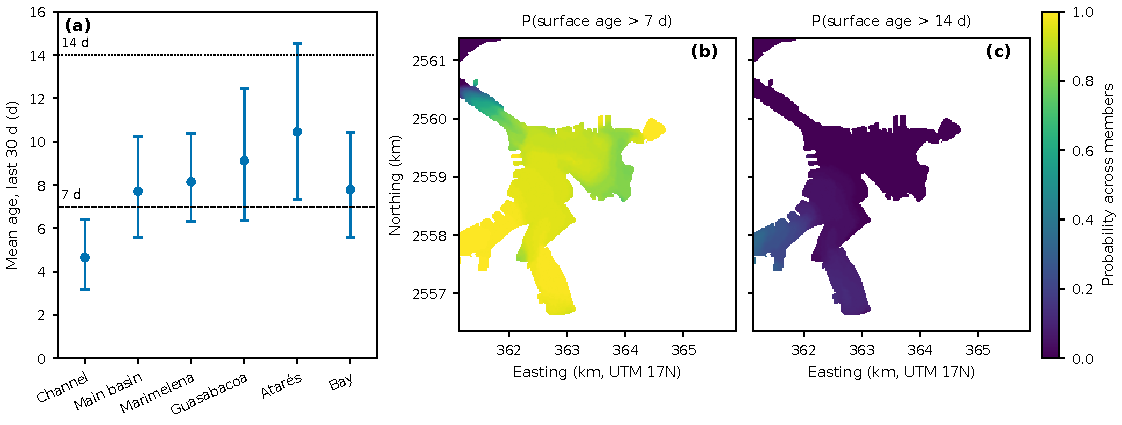
\includegraphics[width=\textwidth]{figuras/fig_ensemble.pdf}
\caption{Water age across the ensemble (128 members of blocks A and B, last 30 of 120
days). (a) Mean age of each zone: median and P5--P95; the dashed and dotted lines are the
7- and 14-day thresholds. (b, c) Probability across members that the surface age exceeds 7
and 14 days.}\label{fig:ens}
\end{figure*}

Table~\ref{tab:concl} gives the verdict on the conclusions fixed in advance. Six of the
seven are robust: the order of the zones (C1, C2, C4), a bay-mean age below one month and
well below four months (C5, C6), and a channel whose surface water is older than its bottom
water (C7), the signature of the estuarine circulation, in every single member. Marimelena
is older than the main basin in only 76\% of the members (C3, fragile), consistent with its
shifting position in the mechanism runs. A bay-mean age above one week is fragile, and above
two weeks or one month it is rejected. All of this holds within the structure that the
ensemble shares: density from salinity only, January--April 2016, and the 2002 river flows
scaled by 0.25--2. The last column of Table~\ref{tab:concl}, discussed in
Section~\ref{sec:res-robust}, tests the most important thing that structure leaves out.

\begin{table*}[!t]
\centering\small
\caption{Conclusions fixed before the results were computed (C, P: metrics protocol,
27 October 2026; R: tracer protocol, 8 November 2026) and their outcome. ``Holds in'' is the
fraction of the 128 members of blocks A and B, or the number of the four tracer cases. The
last column repeats the test with the air--sea heat flux and OISST temperature: in the
16-member subset for C1--C8 and P, and in tracer case T3 for R1--R4
(Section~\ref{sec:res-robust}). Case T1 failed the tracer-budget check of the protocol;
R1--R4 hold with both transport-solver tolerances (Section~\ref{sec:extra}).}\label{tab:concl}
\begin{tabular}{lp{9.6cm}rll}
\toprule
& Conclusion & Holds in & Class & With heat flux\\
\midrule
C1 & Mean age increases from channel to basin to Guasabacoa to Atar\'es & 1.00 & Robust & Robust\\
C2 & Atar\'es is older than the channel & 1.00 & Robust & Robust\\
C3 & Marimelena is older than the main basin & 0.76 & Fragile & Robust (1.00)\\
C4 & Guasabacoa and Atar\'es are older than the main basin & 1.00 & Robust & Robust\\
C5 & Bay-mean age is below 30 days & 1.00 & Robust & Robust\\
C6 & Bay-mean age is below 120 days (the ``four months'' of \citealt{JICA2004}) & 1.00 & Robust & Robust\\
C7 & In the channel, surface water is older than bottom water (estuarine circulation) & 1.00 & Robust & Robust\\
P & Bay-mean age exceeds 7 days & 0.68 & Fragile & Robust\\
P & Bay-mean age exceeds 14 days & 0 & Rejected & Fragile (0.44)\\
P & Bay-mean age exceeds 30 days & 0 & Rejected & Rejected\\
C8 & Input with the largest total Sobol index for the bay-mean age: river discharge & -- &
Reported & Discharge$^{a}$\\
\midrule
R1 & The water of each river is renewed in less than 7 days ($T_i < 7$~d) & 4 of 4 & Robust & Holds (T3)\\
R2 & River water is a smaller fraction of the volume of Atar\'es than of Guasabacoa & 4 of 4 & Robust & Holds (T3)\\
R3 & Most of the Luyan\'o and Mart\'in P\'erez water in the bay is in Guasabacoa and the
main basin ($>50$\% of $M_i$) & 4 of 4 & Robust & Holds (T3)\\
R4 & Most of the Tadeo water in the bay is in Marimelena ($>50$\% of $M_\mathrm{Tadeo}$) & 0 of 4 & Rejected & Fails (T3)\\
\bottomrule
\multicolumn{5}{l}{\footnotesize $^{a}$ Largest Spearman correlation with the bay-mean age
($\rho = -0.80$); not separable from the tidal amplitude factor with 16 members.}\\
\end{tabular}
\end{table*}

\subsection{River discharge is the unknown that matters}\label{sec:res-sobol}
One input dominates (Fig.~\ref{fig:sobol}). For the bay-mean age, river discharge has a
total Sobol index $S_T = 0.67$ (0.49--0.89) and a first-order index $S_1 = 0.86$
(0.80--0.90), and it leads in every zone ($S_T$ 0.56--0.70). Next, a long way behind, comes
the chart-error field ($S_T$ 0.09--0.14), then, for the whole bay, the wind direction (0.05)
and the choice of survey (0.03). The dredging state, the datum, the bottom drag, the wind
speed and the tidal amplitude all have $S_T \le 0.013$. Two cautions come with $N = 64$. The
first-order indices of the inputs with no effect have intervals of about $\pm0.3$ and only
tell us that they cannot be distinguished from zero; and $S_T$ below $S_1$ for the
discharge is estimator noise, since $S_T \ge S_1$ in theory \citep{Saltelli2008} and the
intervals overlap. A small $S_T$ means that an input cannot be told apart from zero in this
design, not that it is irrelevant.

The ranking does not depend on the sample size (Fig.~\ref{fig:sobolconv}). Recomputed with
the first $N = 16$ and 32 rows of each Saltelli block (176 and 352 members), river discharge
has the largest $S_T$ for the bay-mean age at every $N$ (0.70, 0.61 and 0.68 for $N = 16$,
32 and 64) and in every zone (0.46--0.72), with $S_1 = 0.84$--0.86. The chart-error field
ranks second for $N = 32$ and 64; for $N = 16$ it swaps places with the wind direction,
within overlapping intervals. A given-data estimate of the first-order indices from the 128
members of blocks A and B (eight quantile bins, against a permutation null) confirms the
dominance of discharge ($S_1 = 0.83$; 95th percentile of the null 0.12). Among the other
continuous inputs only the bottom drag slightly exceeds its null (0.13 against 0.105), as
expected by chance among seven tests and consistent with its $S_T$ of 0.007.

\begin{figure*}[!t]
\centering
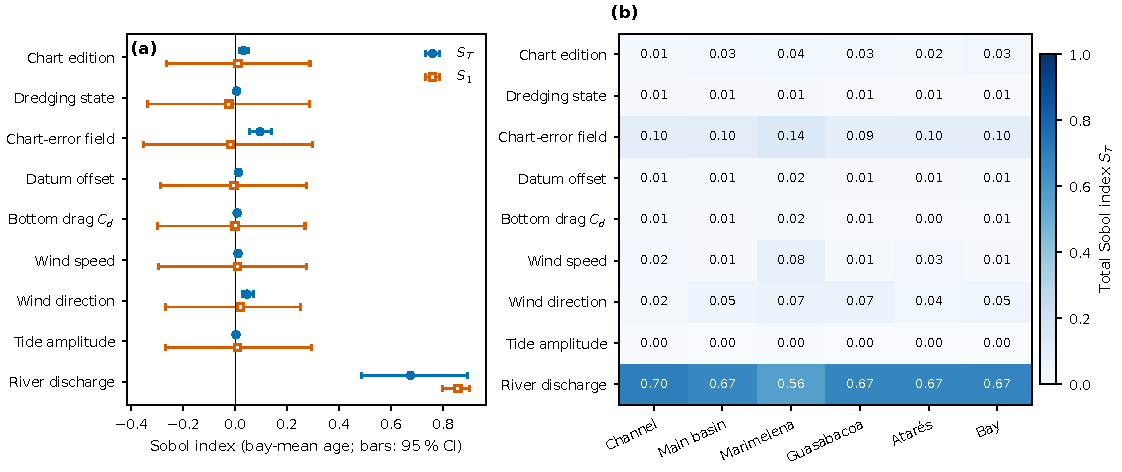
\includegraphics[width=\textwidth]{figuras/fig_sobol.pdf}
\caption{Sobol sensitivity of the mean water age (Jansen estimators, $N = 64$, 704
members). (a) First-order ($S_1$) and total ($S_T$) indices for the bay-mean age, with 95\%
bootstrap intervals (1000 resamples). (b) Total index of each input for each zone and the
whole bay.}\label{fig:sobol}
\end{figure*}

\subsection{Where the river water goes}\label{sec:res-fate}
The water of each river leaves the bay within days (Fig.~\ref{fig:fate}). Its renewal time
$T_i$ is 1.7--2.5~days in the central case and 1.3--5.7~days over the four cases, the
longest being the Tadeo with a quarter of its discharge, so R1 holds everywhere. More
discharge means faster renewal, as expected when the rivers themselves drive the exchange.
In five of the twelve river--case pairs $M_i$ was still drifting, by $-2.3$ to $+1.5$\% per
day, which adds to the numerical uncertainty of $T_i$.

The Luyan\'o and Mart\'in P\'erez water spreads from the head of Guasabacoa into the main
basin: 63--64\% and 67--69\% of it, respectively, lies in Guasabacoa and the main basin in
all four cases (R3). In every case the river-water fraction of Atar\'es is lower than that
of Guasabacoa, but only by 6--11\% in relative terms (R2). The Tadeo is the surprise. It
enters on the shore of Marimelena, yet only 10--15\% of its water in the bay stays there,
against 44--48\% in the main basin, so R4 is rejected in all four cases.

\begin{figure*}[!t]
\centering
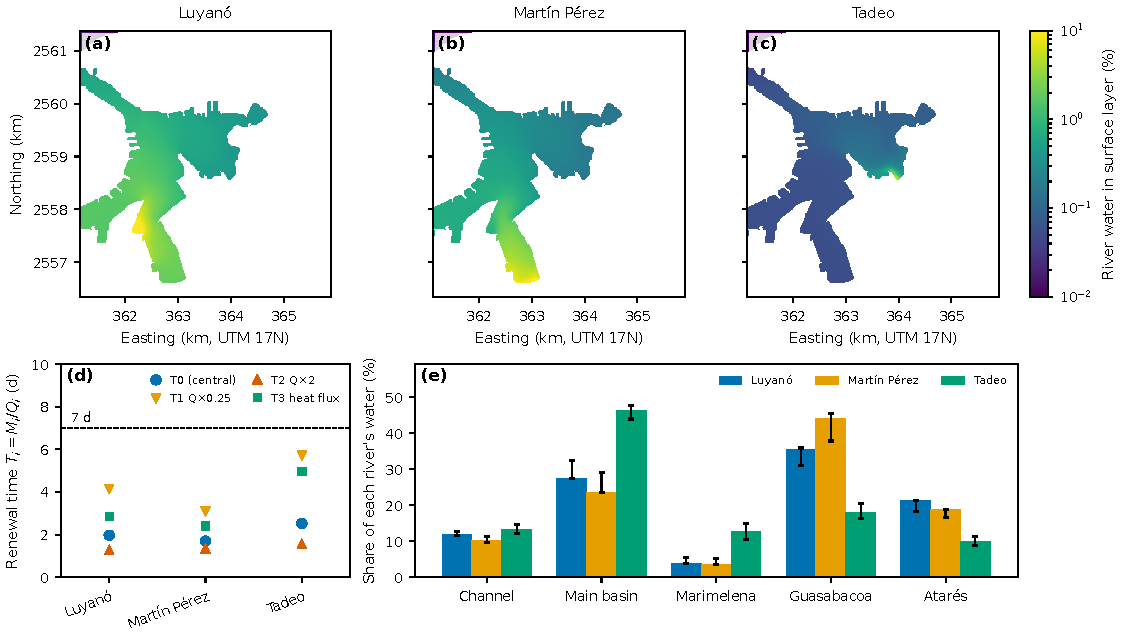
\includegraphics[width=\textwidth]{figuras/fig_rivers.pdf}
\caption{Water of each river in the bay. (a--c) Fraction of river water in the surface
layer, case T0, last 30 days: (a) Luyan\'o, (b) Mart\'in P\'erez, (c) Tadeo (logarithmic
scale). (d) Renewal time $T_i = M_i/Q_i$ of each river in the four cases; the dashed line
is the 7-day threshold of R1. (e) Share of the water of each river in the bay that lies in
each zone, case T0; bars show the range of the four cases.}\label{fig:fate}
\end{figure*}

\subsection{The air--sea heat flux outweighs every sampled input}\label{sec:res-robust}
How turbulence and vertical resolution are represented hardly matters
(Table~\ref{tab:robust}, Fig.~\ref{fig:heat}). With the $k$--$\varepsilon$ closure, twice
as many levels or ten times more background mixing, the bay-mean age stays at
6.6--7.5~days, the channel keeps its older surface water, and the zones keep their order.

The air--sea heat flux is different. Over 120 days, with the ERA5 heat flux and a boundary
fixed at 28~$^\circ$C, the bay-mean age rises to 16.8~days and the surface--bottom contrast
in the channel largely disappears; that boundary was up to 3.5~$^\circ$C too warm. With the
daily OISST temperature the bay-mean age reaches 11.2~days over days 90--120 and is still
rising ($+0.24$~d\,d$^{-1}$), while the channel keeps an older surface (10.0~days) than
bottom (6.6~days) and the zones keep their order. Neither run moves smoothly towards a steady
value (Fig.~\ref{fig:heat}): with OISST the age climbs to about 20~days by early March,
falls to about 8~days within two weeks and rises again, whereas all the runs without heat
flux stay between about 5 and 10~days after the first month.

The two later tests show that this is not a slow start. Over a full year, the base run
settles at 6.57~days (drift $-0.03$~d\,d$^{-1}$), but with the heat flux and OISST the
bay-mean age oscillates between about 5 and 21~days (30-day means) and averages 15.4~days
over the last 30 days of the year, still rising ($+0.55$~d\,d$^{-1}$; channel 10.4~days,
Atar\'es 18.2~days); the run with the 28~$^\circ$C boundary gives 16.7~days, also rising.
In the 16-member subset, the median bay-mean age rises from 7.4~days (5.9--10.4 between the
5th and 95th percentiles) without heat flux to 13.8~days (9.2--17.7) with it. It is higher
in all 16 members, and no member reaches the equilibrium criterion, against 14 of 16 without
heat flux. The shift of the median, 6.4~days, is larger than the whole 90\% range of the
main ensemble (4.8~days): one structural choice moves the answer further than all nine
sampled inputs together.

The robust conclusions survive it (Table~\ref{tab:concl}, last column). The channel remains
the youngest zone in every member, its surface water stays older than its bottom water, and
the bay-mean age stays below one month. River discharge remains the input most strongly
correlated with age (Spearman $\rho = -0.80$), although with 16 members it cannot be
separated from the tidal amplitude factor, which is collinear with it in this subset
(partial $\rho = -0.39$). Three verdicts change: Marimelena becomes older than the main basin
in every member, an age above one week becomes robust, and an age above two weeks becomes
fragile (0.44). In the tracer case with the heat flux (T3) R1--R3 hold and R4 fails, as in
the other cases. A plausible reason for the longer age is that cooling makes the water of
the shallow bay denser, as differential cooling does in the shallow margins of lakes
\citep{Doda2022}, and works against the buoyancy of the river water; we did not identify the
events that build up and reset the age in the heat-flux runs.

\begin{figure}[!t]
\centering
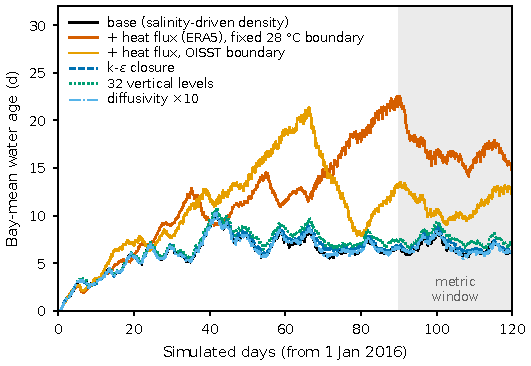
\includegraphics[width=\columnwidth]{figuras/fig_robustness.pdf}
\caption{Bay-mean water age in the central member with rivers over the first 120 days of
2016, under changes of model structure: base (salinity-driven density), $k$--$\varepsilon$
closure, 32 vertical levels, ten times larger background diffusivity, and the ERA5 air--sea
heat flux with the open boundary fixed at 28~$^\circ$C or at the daily OISST temperature.
The shaded band is the 30-day window of the metrics.}\label{fig:heat}
\end{figure}

\begin{table*}[!t]
\centering\small
\caption{Sensitivity of the density-driven circulation to the model structure: mean water
age (days) over days 90--120 of the central member with rivers.}\label{tab:robust}
\footnotesize\setlength{\tabcolsep}{4pt}
\begin{tabular}{lrrrrrr}
\toprule
& Base & $k$--$\varepsilon$ & 32 lev. & Diff.\,$\times10$ & Heat, 28\,$^\circ$C &
Heat, OISST\\
\midrule
Channel & 4.0 & 4.4 & 4.9 & 4.1 & 11.5 & 7.6\\
Main basin & 6.7 & 7.0 & 7.5 & 6.7 & 17.9 & 11.8\\
Marimelena & 7.0 & 7.1 & 7.5 & 7.1 & 19.3 & 12.9\\
Guasabacoa & 7.6 & 8.0 & 8.7 & 7.6 & 18.1 & 12.1\\
Atar\'es & 8.8 & 9.4 & 10.0 & 8.8 & 19.5 & 13.3\\
Whole bay & 6.6 & 6.9 & 7.5 & 6.6 & 16.8 & 11.2\\
Trend (d\,d$^{-1}$) & $+0.02$ & $+0.01$ & $+0.01$ & $+0.03$ & $-0.10$ & $+0.24$\\
Channel sfc./bot. & 6.6/1.8 & 6.7/2.1 & 7.5/2.3 & 6.6/1.9 & 14.2/10.6 & 10.0/6.6\\
\bottomrule
\end{tabular}
\end{table*}

\subsection{Sentinel-2 agrees, but so would chance}\label{sec:res-s2}
The surface fresh water of the run with rivers correlates with the persistence of turbidity
anomalies, $\rho = 0.45$ (0.35--0.54) over 8908 pixels in 145 blocks, so the registered
prediction holds (Fig.~\ref{fig:s2}). The shift control, however, takes the result away: 5\%
of the shifted satellite maps give correlations of 0.61 or more, and 16\% beat the observed
value ($p = 0.16$). Under the rule registered beforehand, the agreement cannot be
distinguished from spatial chance. The age fields of the runs with rivers, with tide and
wind, and with the tide alone behave the same way ($\rho$ = 0.46, 0.48 and 0.29;
$p$ = 0.15--0.28). Both maps simply increase from the mouth towards the heads of the coves,
and any field with that gradient matches the satellite record. Across the ensemble $\rho$ is
positive in all 128 members (median 0.45, P5--P95 0.43--0.47), but this says only that the
pattern hardly depends on the inputs. Sentinel-2 thus confirms the broad mouth-to-head
gradient and nothing more.

One pattern was noticed only after the test and is reported as exploratory: the satellite
frequency is highest towards the heads of the Guasabacoa and Atar\'es coves, and only the
former has a modelled river. The diagnostics of the companion study do not settle the cause:
in Guasabacoa the signal behaves like land adjacency \citep{Sterckx2011}, and in Atar\'es
piers lie 30--52~m away, which may mean berthed vessels. Discharges missing from
OpenStreetMap and from the 2002 values, or resuspension in shallow water, are not excluded
but are not supported by the satellite data. The modelled rivers do not account for it by
themselves: they put a little less of their water into Atar\'es than into Guasabacoa (R2).

\begin{figure*}[!t]
\centering
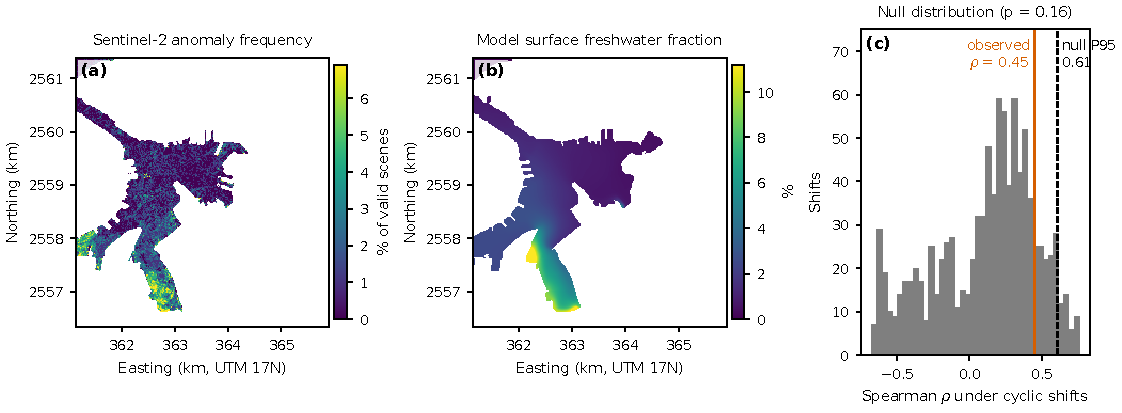
\includegraphics[width=\textwidth]{figuras/fig_sentinel2.pdf}
\caption{Comparison with Sentinel-2. (a) Frequency of positive turbidity anomalies,
2017--2025 (\% of valid scenes; companion study, \ph{link\_sentinel2}). (b) Modelled surface
freshwater fraction at 16:00~UTC, last 30 days of the mechanism run with rivers.
(c) Spearman $\rho$ between the two maps under 999 cyclic shifts of the satellite map by at
least 500~m; the solid line is the observed $\rho = 0.45$ and the dashed line the 95th
percentile of the shifts (0.61).}\label{fig:s2}
\end{figure*}

%======================================================================
\section{Discussion}\label{sec:discussion}
%======================================================================
\subsection{Parametric and structural uncertainty}\label{sec:disc-unc}
Some answers survive everything we sampled. The tide alone renews the bay poorly; an
estuarine circulation runs through the channel; the bay is renewed in less than a month and
far less than four months; water gets older from the channel towards Atar\'es; and each
river's water leaves within days. Other answers do not survive: whether the bay-mean age
exceeds a week (68\% of members), whether Marimelena is older than the main basin, and the
tail of Atar\'es beyond two weeks (11\%). Ages above two weeks for the whole bay, and the
idea that the Tadeo water stays in Marimelena, are rejected.

These verdicts hold within the structure that the ensemble shares, and the heat flux shows
how much that qualification matters. The 90\% range of the ensemble, 5.6--10.4~days, is the
uncertainty that comes from the nine inputs. Adding one process that the ensemble leaves
out shifts the median by more than that whole range, raises the age in every member tested
and keeps it from settling. Read on its own, the spread of a parametric ensemble would have
suggested more confidence than the model can support. This is the practical meaning of the
distinction between input and structural uncertainty
\citep{Walker2003,Refsgaard2006,Gupta2012}: a Sobol analysis ranks the uncertainties that the
modeller has put into the design, and only tests of the structure reveal those left outside
it.

The two kinds of test are also complementary in what they leave standing. The conclusions
that are robust in the ensemble and survive the heat flux, the order of the zones, the
estuarine circulation in the channel, an age below one month and the leading role of
discharge, are the ones we would defend without measurements. The ones that change with the
heat flux, whether the bay exceeds one or two weeks and whether Marimelena is older than
the main basin, depend on a process that needs its own data. The safest summary therefore
has two parts: about one week without the heat flux and about two weeks, not stationary, with
it. In both cases the bay is renewed in weeks rather than months, faster where the river
water flows out and slower in Atar\'es.

\subsection{Why a tidal estimate misleads here}
The prism estimate puts renewal at about three weeks, and the model falls on either side of
it depending on what drives the flow. With the tide alone the bay is much slower (166~days,
still rising): nearly all the water that leaves on the ebb comes back, so the real
return-flow factor is close to one \citep{Sanford1992}. With rivers and density the bay is
much faster (about a week), because the exchange is carried by a gravitational circulation
that a prism does not contain \citep{MacCready2010}. The estimate gets the diagnosis right,
that the tide alone does little, but neither of its numbers describes the bay. In a
small-tide bay behind a narrow channel, a tidal estimate is a poor guide in both directions.

\subsection{The four months of earlier work}\label{sec:jica}
The only earlier figure for the bay is a freshwater retention time of about four months
\citep{JICA2004}. It cannot be set directly against water age, which counts river water as
new water. The comparable quantity is the freshwater flushing time $T_f$. In the runs with
full fields, fresh water makes up 1.1--1.2\% of the bay volume (2.3--2.5\% at the surface),
which gives $T_f \approx 1.8$--2.0~days, or 4.2~days with the heat flux and the
28~$^\circ$C boundary. The renewal times of the three rivers (1.3--5.7~days,
Section~\ref{sec:res-fate}) agree. The gap with four months is therefore larger than the
comparison with age suggests, about a factor of 60. In the model the river water leaves
quickly in the surface layer; the bay-mean age is longer than $T_f$ because it also follows
the sea water entering near the bottom.

The report does not give its method. With its own volume of 47~hm$^3$, four months would
correspond to the bay volume divided by an inflow of about 4.5~m$^3$\,s$^{-1}$, that is, to
a renewal with no exchange with the sea; we cannot confirm that this was the calculation.
The real inflow, which includes unmeasured sewage and drains, and the evaporation and
precipitation missing from the model could also contribute. The heat flux, the largest
effect we found, raises the bay-mean age only to about two weeks (13.8~days in the
16-member subset, and 30-day means never above 21~days over a full year), still at least
five times shorter than four months.

\subsection{What to measure first}
Two measurements stand out, one for each kind of uncertainty. Among the inputs, river
discharge carries most of the variance of the age in every zone, and the
2.14~m$^3$\,s$^{-1}$ used here are a single set of 2002 values that does not include sewage
or drains. This ranking is conditional on the ranges of Table~\ref{tab:params}: the
discharge factor ranges over a factor of eight, whereas the tide and wind factors span
$\pm$10--20\%. It shows which of the present uncertainties matter most, not which processes
matter most. Gauging the three rivers and the main outfalls would reduce the uncertainty more
than any new survey of the bay. Bathymetry comes second, through the chart error; the choice
of survey, the dredging, the datum, the bottom drag and the tidal amplitude matter little
for water age. For the structure, a temperature and salinity record in the bay, with
profiles in the channel, would constrain the heat flux, the largest effect outside the
ensemble, and show directly whether the estuarine circulation on which the robust
conclusions rest (C7) exists.

\subsection{Limitations}
The bathymetry comes from surveys more than a century old; the dredging state and the chart
error bound that uncertainty but do not remove it. In the ensemble, density depends on
salinity only. The heat flux was tested in the central member and in a 16-member subset,
without a Sobol analysis, so we do not know how it interacts with the inputs. Net
evaporation minus precipitation in the dry season is of the order of 0.1~m$^3$\,s$^{-1}$,
about 5\% of the river inflow (rough estimate), although evaporation can reverse the
density contrast of shallow bays with little river flow \citep{Largier1997}. All ensemble
runs cover January--April 2016, in the dry season, with no interannual variability. Wind
explains little of the variance of the age ($S_T$ 0.011 for its speed and 0.046 for its
direction), so the choice of year is unlikely to change the ensemble conclusions; the heat
flux and sea temperature, which do depend on the year, enter only the structural tests,
which are therefore specific to 2016. River flows come from one set of 2002 values, and the
sewage load is unmeasured. ERA5 resolves the area with a few grid points and misses local
wind effects. The transport-solver tolerance adds a numerical uncertainty of about 5\% to
water age: rerunning the central case with a $10^5$-fold stricter tolerance raised the
bay-mean age by 5\%, lowered $T_f$ by 3\% and left the Sentinel-2 $\rho$ and R1--R4
unchanged, which is small next to the ensemble spread; in the tracer cases it moved $T_i$ by
up to about $\pm20$\% (Section~\ref{sec:extra}). The discharge through the channel cannot be
used as a result, since besides its sampling error it shows intermittent high-frequency
bursts of unexplained origin, so the model is not checked against the tidal prism in terms
of flux. With $N = 64$ the first-order Sobol indices have wide intervals. And no local
observation constrains the model: the results describe what public data allow, not a
calibrated reconstruction of the bay.

\subsection{Transferability}
The whole chain uses public data (nineteenth-century charts, GEBCO, OpenStreetMap, ERA5,
EOT20 and OISST) and open-source code, with protocols fixed before the results they govern.
The same steps apply to other bays without surveys or gauges: digitise the best historical
charts, estimate their error from overlapping surveys, force the model with global products,
let a variance-based ensemble separate what the data can support from what they cannot
\citep{Pianosi2016,Razavi2021}, and test the conclusions again under the main structural
simplifications. In Havana Bay, the inputs a modeller without data would worry about most,
the century-old charts, the dredging and the tide, barely matter for water age, while a
river discharge measured once in 2002 controls it among the inputs and the air--sea heat
flux outweighs them all. That ranking belongs to a small-tide bay with a narrow channel; the
procedure that produced it does not.

%======================================================================
\section{Conclusions}\label{sec:conclusions}
%======================================================================
We asked what can be known about the renewal of Havana Bay from public data alone.

\begin{enumerate}[label=(\arabic*),leftmargin=2.2em,itemsep=0pt]
\item The tide alone leaves a bay-mean age of 166 days, and wind 97 days. The density
contrast of 2~m$^3$\,s$^{-1}$ of river water brings it down to 6.6 days through an estuarine
circulation, which is robust to the turbulence closure, the resolution and the mixing.
\item Within the ensemble the bay-mean age is about a week (median 7.8 days, P5--P95
5.6--10.4), never above 14 days, and water gets older from the channel to Atar\'es in every
member. Whether the bay exceeds one week, and whether Marimelena is older than the main
basin, remain open.
\item River discharge controls most of the uncertainty that comes from the inputs
($S_T = 0.67$, stable from $N = 16$ to 64); the nineteenth-century charts, the dredging and
the tide matter much less. Gauging the rivers and the sewage outfalls is the first
measurement to make.
\item The air--sea heat flux, left out of the ensemble, matters more than all nine inputs:
in a 16-member subset it raises the median bay-mean age from 7.4 to 13.8 days, in every
member, and keeps it from settling, while the order of the zones and the estuarine
circulation survive. The bay is renewed in about one week without it and about two weeks
with it, in weeks rather than months, and a temperature and salinity record in the bay is
the first measurement for the model structure.
\item The water of each river is renewed in less than six days in four configurations, and
the Tadeo water does not stay in Marimelena. The modelled fresh water matches the Sentinel-2
turbidity record no better than spatial chance, and the freshwater flushing time of about
two days is some 60 times shorter than the four months of the earlier report.
\end{enumerate}

%======================================================================
\section*{Software availability}
\noindent\textit{Name of software:} \ph{nombre\_repositorio}\par
\noindent\textit{Description:} Scripts that download the public inputs, digitise the
charts, build the bathymetry and mesh, generate and run the 704-member SCHISM ensemble on
a Slurm cluster, and post-process the results, with the three analysis protocols.\par
\noindent\textit{Developers:} Alex M. Rivera-Rivera et al.\par
\noindent\textit{Contact:} alex.rivera.rivera@ulb.be\par
\noindent\textit{Language:} Python, Bash, Fortran (SCHISM, Apache~2.0)\par
\noindent\textit{Software required:} SCHISM (commit 09f407e8), Python, Bash, Slurm\par
\noindent\textit{Hardware required:} a Slurm cluster for the ensemble (about 76 core-hours
per member)\par
\noindent\textit{Availability and cost:} free and open source, MIT licence\par
\noindent\textit{Source code:} \ph{link\_repositorio}

\section*{Data availability}
All inputs are public (Table~\ref{tab:data}); each download is recorded with its date in
the repository (\ph{link\_repositorio}). The repository also holds the post-processed
outputs of the ensemble, the mechanism, structural and tracer runs, the design of the
ensemble, and the three analysis protocols with their dated version history. The commits
that fixed the protocols are 773b9fb (Sentinel-2 comparison, 21 October 2026), 231696a (its
shift control, 26 October), 4564b7e (ensemble metrics, committed on 26 October and approved
on 27 October) and 3907fd7 (river tracers, 8 November). The Sentinel-2 turbidity product is
not part of it: its processing and its definition of a turbidity anomaly are described in a
companion study, with its own repository (\ph{link\_sentinel2}).

\section*{Declaration of competing interest}
The authors declare that they have no known competing financial interests or personal
relationships that could have appeared to influence the work reported in this paper.

\section*{Funding}
This work was supported by ARES, with funding from the Belgian Development Cooperation,
through the project ``In situ monitoring of water quality in Cuban bays: creating and
promoting the use of a scientific toolbox''. A.C. and S.C.N. acknowledge funding from the
European Union's Horizon Europe research and innovation programme under grant agreement
No.~101181363 (BioDiMoBot).

\section*{Declaration of generative AI and AI-assisted technologies in the manuscript
preparation process}
During the preparation of this work the authors used Claude (Anthropic) and ChatGPT
(OpenAI) to check numerical consistency, to help write the code that draws the figures, and
to review and edit the language. After using these tools, the authors reviewed and edited
the content as needed and take full responsibility for the content of the published
article.

\section*{Acknowledgements}
Computational resources have been provided by the Consortium des \'Equipements de Calcul
Intensif (C\'ECI), \linebreak[1] funded by the Fonds de la Recherche Scientifique de Belgique
(F.R.S.-FNRS) under Grant No.\ 2.5020.11 and by the Walloon Region. All simulations
were run on the Lemaitre4 cluster of C\'ECI.

\printcredits

\bibliographystyle{cas-model2-names}
\bibliography{referencias}

%======================================================================
% Supplementary material: to be submitted as a separate file.
\clearpage
\onecolumn
\section*{Supplementary material}
\setcounter{figure}{0}
\renewcommand{\thefigure}{S\arabic{figure}}
\renewcommand{\theHfigure}{S\arabic{figure}}
\setcounter{table}{0}
\renewcommand{\thetable}{S\arabic{table}}
\renewcommand{\theHtable}{S\arabic{table}}

\begin{figure}[!h]
\centering
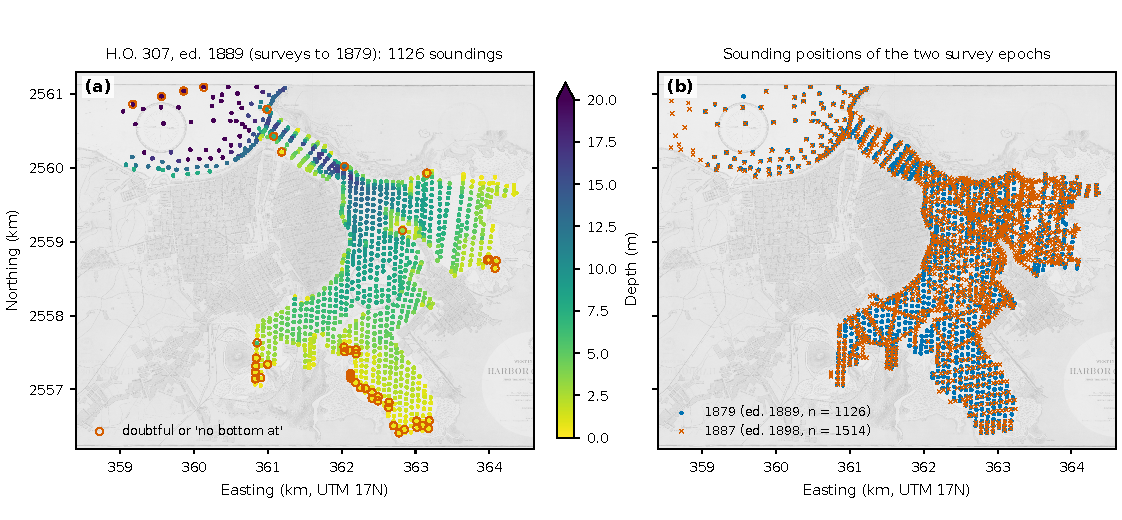
\includegraphics[width=\textwidth]{figuras/figS_soundings.pdf}
\caption{Digitised soundings of chart No.~307. (a) The 1126 soundings of the 1889 edition
(surveys to 1879), coloured by depth; circles mark doubtful readings and ``no bottom at''
entries. (b) Positions of the 1879 (1889 edition, 1126) and 1887 (1898 edition, 1514)
soundings. The 1887 soundings are drawn on the 1889 chart, printed from the same
plate.}\label{fig:soundings}
\end{figure}

\begin{figure}[!h]
\centering
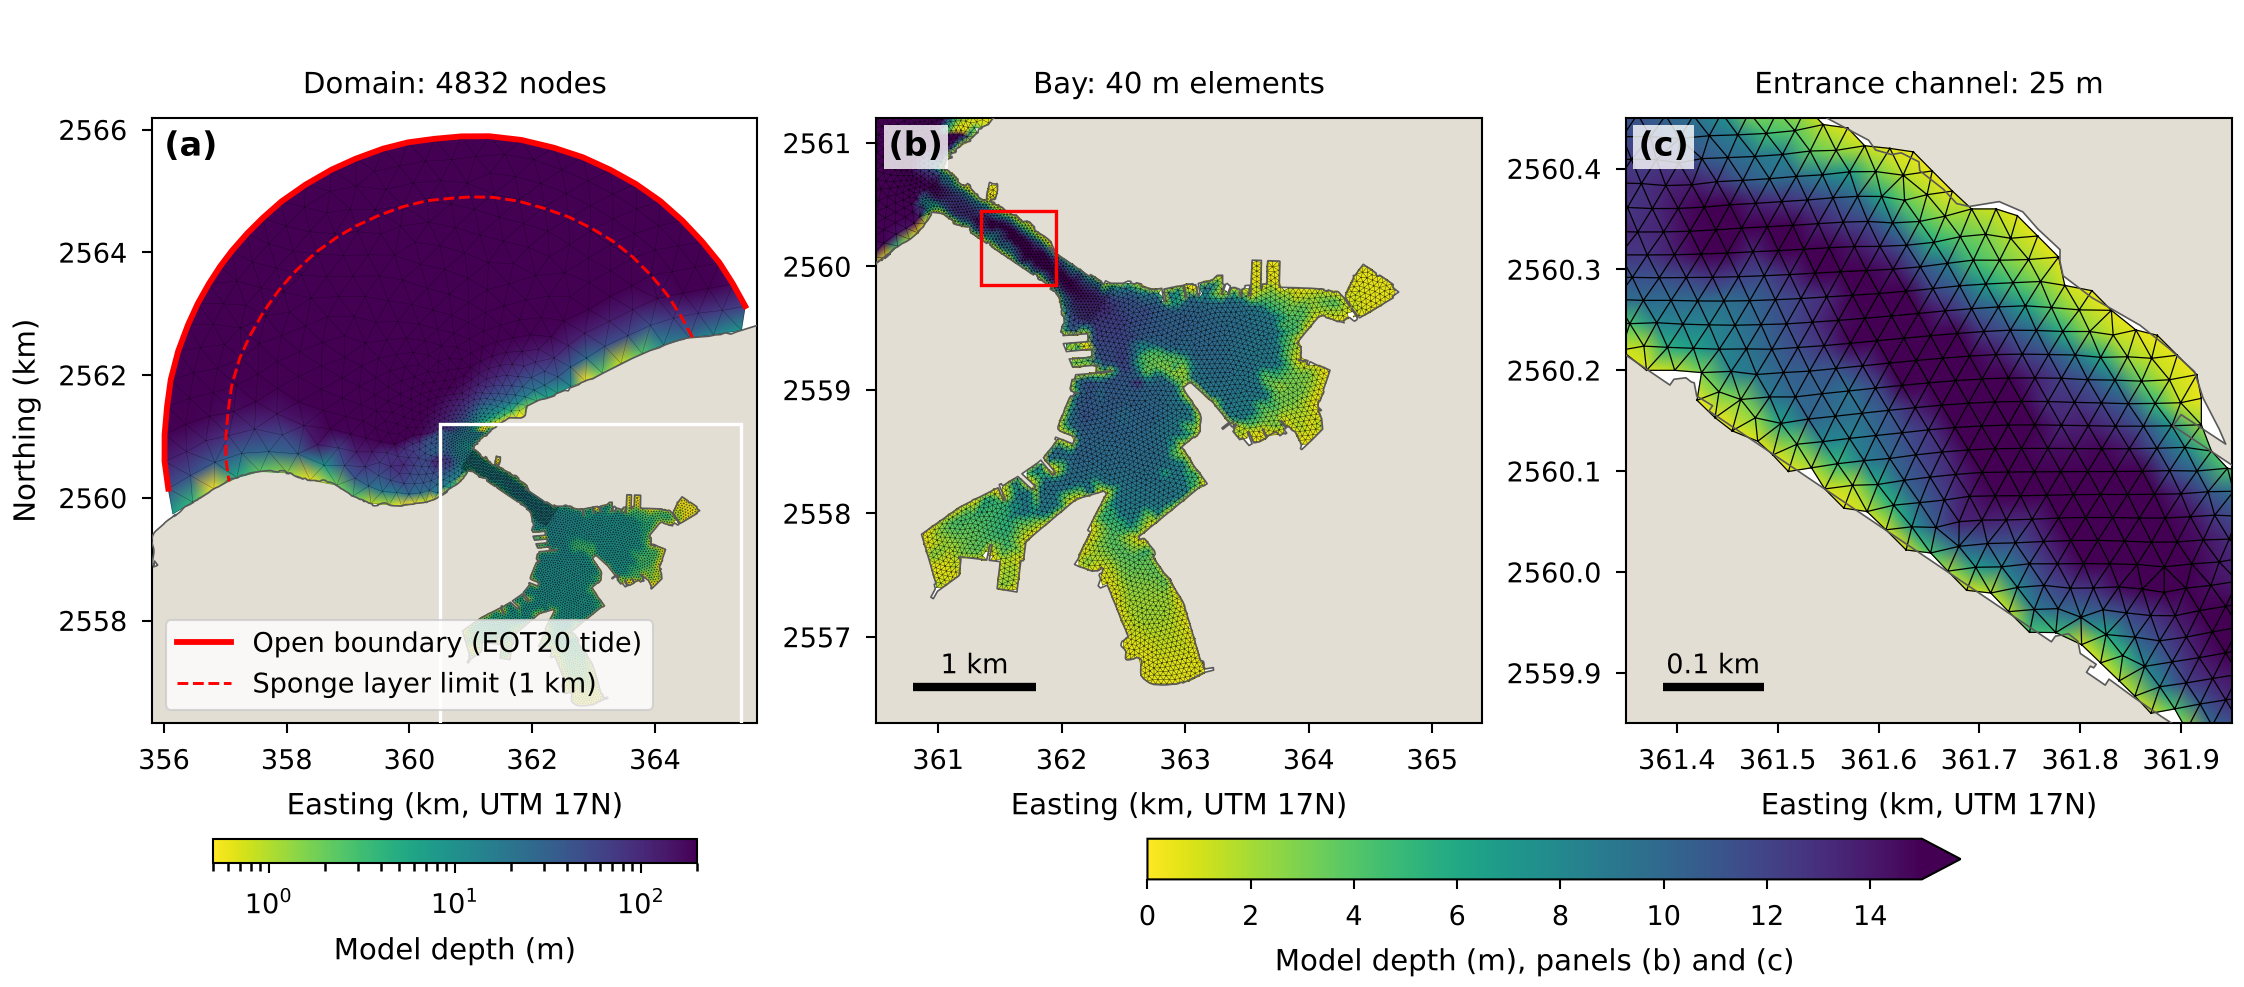
\includegraphics[width=\textwidth]{figuras/fig03_mesh.png}
\caption{Model mesh (4832 nodes, 8941 triangles), coloured by model depth. (a) Whole domain,
with the open boundary forced by the EOT20 tide and the inner limit of the 1~km sponge
layer. (b) The bay, with 40~m elements. (c) The entrance channel, with 25~m
elements.}\label{fig:mesh}
\end{figure}

\begin{figure}[!h]
\centering
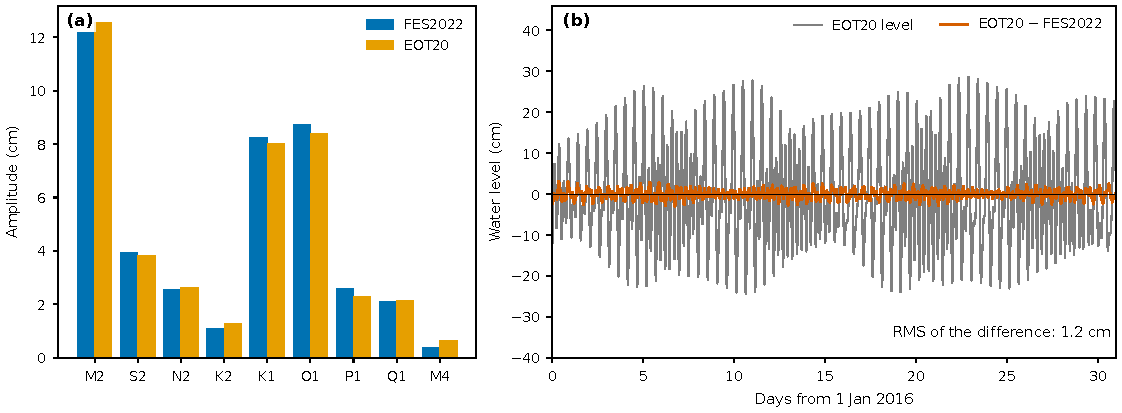
\includegraphics[width=\textwidth]{figuras/fig_tide.pdf}
\caption{Tide off the bay mouth. (a) Amplitudes of nine constituents in FES2022 and EOT20.
(b) Water level predicted with EOT20 and its difference from FES2022, January 2016 (RMS
1.2~cm).}\label{fig:tide}
\end{figure}

\begin{table}[!h]
\centering\small
\caption{Inputs of the Monte Carlo tidal-prism estimate (Section~\ref{sec:eval}), each drawn
from a triangular distribution ($2\times10^5$ samples). The tide is not a distribution: each
sample takes a real day of a year synthesised from the nine EOT20 constituents off the
mouth.}\label{tab:prismS}
\begin{tabular}{llrrrl}
\toprule
Input & Unit & Minimum & Mode & Maximum & Basis\\
\midrule
Bay area & km$^2$ & 4.7 & 4.91 & 5.2 & OpenStreetMap coastline\\
Mean depth & m & 5.2 & 6.2 & 7.3 & Charts, as surveyed to dredged (Section~\ref{sec:bathy})\\
Channel width & m & 220 & 220 & 280 & Harbour pilots, 220--330~m \citep{Practicos2018}\\
Channel section depth & m & 9.0 & 11.0 & 12.8 & 12.8~m axis, shallower margins\\
Return-flow factor $\beta$ & -- & 0.3 & 0.6 & 0.85 & Assumed\\
River inflow & m$^3$\,s$^{-1}$ & 1.0 & 2.14 & 5.0 & 2002 values \citep{JICA2004}, plus sewage\\
\bottomrule
\end{tabular}
\end{table}

\begin{figure}[!h]
\centering
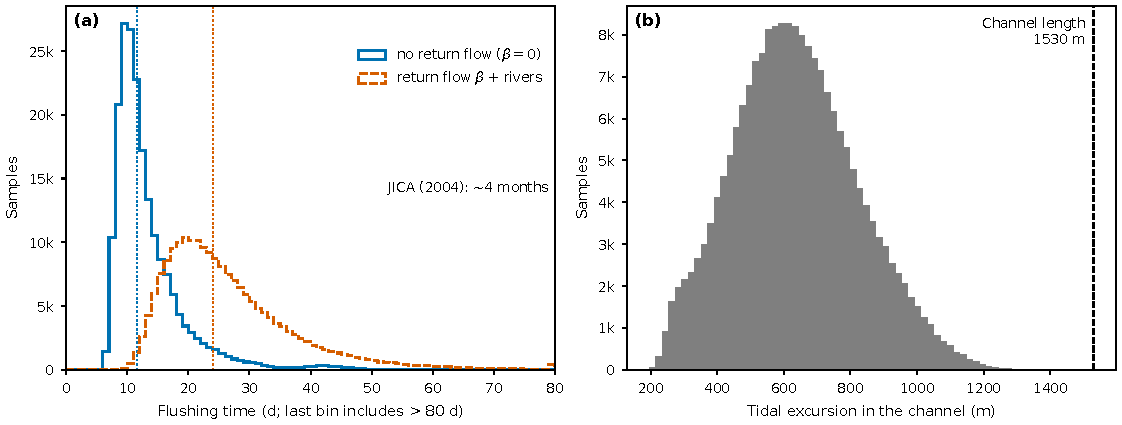
\includegraphics[width=\textwidth]{figuras/fig_prisma.pdf}
\caption{Monte Carlo tidal-prism estimate ($2\times10^5$ samples). (a) Flushing time without
return flow ($\beta = 0$) and with return flow and rivers; the dotted lines mark the
medians; the label marks the earlier estimate of about four months \citep{JICA2004}, far beyond the axis.
(b) Tidal excursion in the channel against the channel length of 1530~m.}\label{fig:prisma}
\end{figure}

\subsection*{Text S1. Numerical behaviour of the ensemble}
A 20-day segment takes 0.65--9~h of wall time (median 1.6~h); the cost of 76 core-hours
per member was estimated from 484 members. The largest model speeds are spurious and do not
affect the results (Fig.~\ref{fig:boundary}). In 94\% of the members the maximum
depth-averaged speed (median 6.0~m\,s$^{-1}$) sits on the open boundary, 4--5~km from the
mouth, where the model depth is capped at 200~m. These speeds did not appear in a 10-day
rerun of the central member (maximum 1.8~m\,s$^{-1}$ in the same region), and we did not
isolate their cause; they are capped by the velocity limiter of SCHISM
(5~m\,s$^{-1}$ per component). Inside the bay, 68 members exceed 3~m\,s$^{-1}$ at a few
nodes only 0.3--0.5~m deep, where SCHISM caps the velocity. Neither is related to the
bay-mean age (Spearman $\rho = -0.07$ and $-0.04$), and removing the 15 such members of
blocks A and B changes no class (bay-mean age 7.73 instead of 7.78~days).

\begin{figure}[!h]
\centering
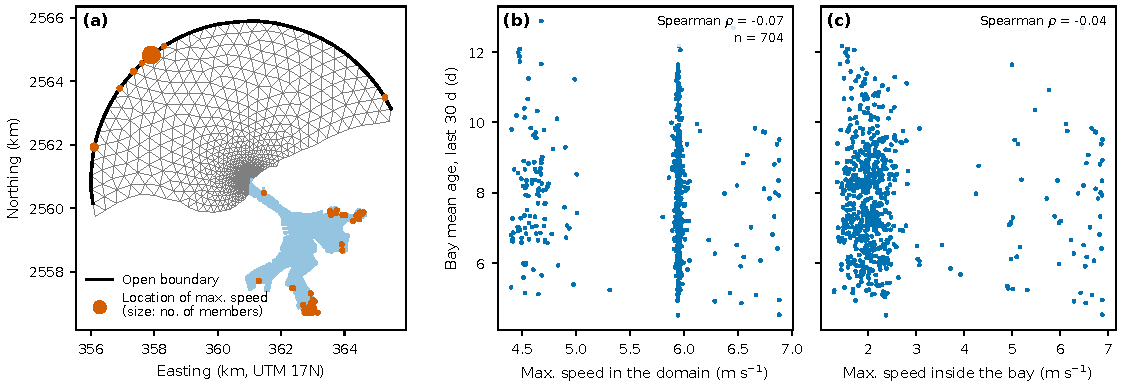
\includegraphics[width=\textwidth]{figuras/figS_boundary.pdf}
\caption{Spurious velocities in the 704 members. (a) Location of the maximum
depth-averaged speed of each member (symbol size: number of members). (b) Bay-mean age
against the maximum speed in the domain. (c) Bay-mean age against the maximum speed inside
the bay.}\label{fig:boundary}
\end{figure}

\begin{figure}[!h]
\centering
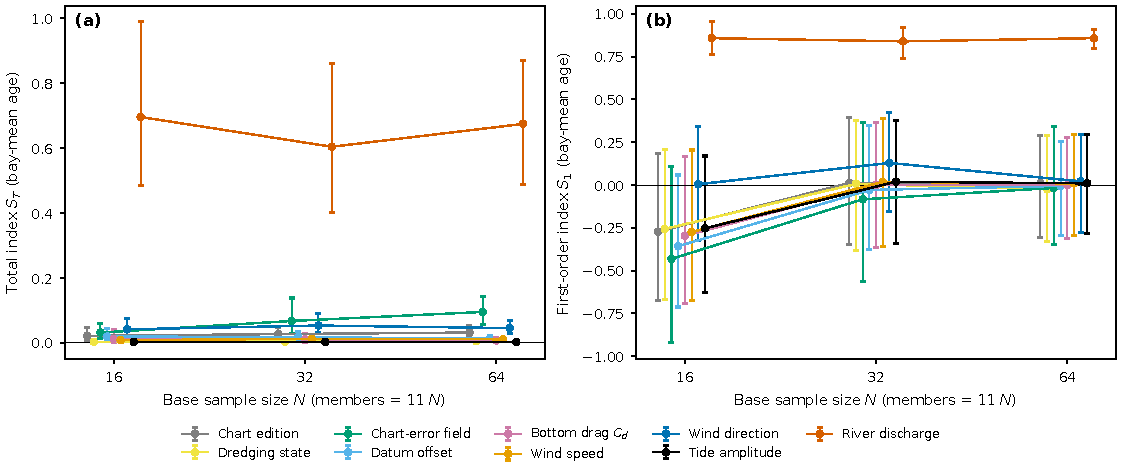
\includegraphics[width=\textwidth]{figuras/figS_sobol_convergence.pdf}
\caption{Convergence of the Sobol indices of the bay-mean age with the base sample size
$N$ (Jansen estimators on the first $N$ rows of each Saltelli block; members $= 11N$).
(a) Total indices $S_T$ and (b) first-order indices $S_1$ of the nine inputs, with 95\%
bootstrap intervals.}\label{fig:sobolconv}
\end{figure}

\end{document}
